
%% 使用 njuthesis 文档类生成南京大学学位论文的示例文档
%%
%% 作者:胡海星,starfish (at) gmail (dot) com
%% 项目主页: http://haixing-hu.github.io/nju-thesis/
%%
%% 本样例文档中用到了吕琦同学的博士论文的提高和部分内容,在此对他表示感谢。
%%
\documentclass[master]{njuthesis}
%% njuthesis 文档类的可选参数有:
%%   nobackinfo 取消封二页导师签名信息。注意,按照南大的规定,是需要签名页的。
%%   phd/master/bachelor 选择博士/硕士/学士论文

% 使用 blindtext 宏包自动生成章节文字
% 这仅仅是用于生成样例文档,正式论文中一般用不到该宏包
\usepackage[math]{blindtext}

\usepackage{anyfontsize}
\usepackage{algorithm}
\usepackage{algorithmicx}
\usepackage[noend]{algpseudocode}
\usepackage{graphicx}
\usepackage{caption}
\usepackage{subcaption}

%\captionsetup{compatibility=false}
%\usepackage{graphicx,subfigure}
\usepackage{filecontents}
\usepackage{tkz-tab}
%\usepackage{subfig}
\usepackage{tikz}
\usepackage{multirow}
\usepackage{sistyle}
\SIthousandsep{,}
\usepackage{ascii}
\usepackage[T1]{fontenc}
\usepackage{booktabs}% http://ctan.org/pkg/booktabs
\usepackage{makecell}% http://ctan.org/pkg/makecell
\usepackage{tabularx}
\usepackage{bm}

\usepackage{listings}
\usepackage{color}

\definecolor{dkgreen}{rgb}{0,0.6,0}
\definecolor{gray}{rgb}{0.5,0.5,0.5}
\definecolor{mauve}{rgb}{0.58,0,0.82}

\lstset{frame=tb,
  language=Scala,
  aboveskip=3mm,
  belowskip=3mm,
  showstringspaces=false,
  columns=flexible,
  basicstyle={\small\ttfamily},
  numbers=none,
  numberstyle=\tiny\color{gray},
  keywordstyle=\color{blue},
  commentstyle=\color{dkgreen},
  stringstyle=\color{mauve},
  breaklines=true,
  breakatwhitespace=true,
  tabsize=3
  }
%\newtheorem{observation}[theorem]{\textbf{事实}}
%%%%%%%%%%%%%%%%%%%%%%%%%%%%%%%%%%%%%%%%%%%%%%%%%%%%%%%%%%%%%%%%%%%%%%%%%%%%%%%
% 设置《国家图书馆封面》的内容,仅博士论文才需要填写

% 设置论文按照《中国图书资料分类法》的分类编号
\classification{0175.2}
% 论文的密级。需按照GB/T 7156-2003标准进行设置。预定义的值包括:
% - \openlevel,表示公开级:此级别的文献可在国内外发行和交换。
% - \controllevel,表示限制级:此级别的文献内容不涉及国家秘密,但在一定时间内
%   限制其交流和使用范围。
% - \confidentiallevel,表示秘密级:此级别的文献内容涉及一般国家秘密。
% - \clasifiedlevel,表示机密级:此级别的文献内容涉及重要的国家秘密 。
% - \mostconfidentiallevel,表示绝密级:此级别的文献内容涉及最重要的国家秘密。
% 此属性可选,默认为\openlevel,即公开级。
\securitylevel{\controllevel}
% 设置论文按照《国际十进分类法UDC》的分类编号
% 该编号可在下述网址查询:http://www.udcc.org/udcsummary/php/index.php?lang=chi
\udc{004.72}
% 国家图书馆封面上的论文标题第一行,不可换行。此属性可选,默认值为通过\title设置的标题。
\nlctitlea{基于Spark的大规模图数据中的}
% 国家图书馆封面上的论文标题第二行,不可换行。此属性可选,默认值为空白。
\nlctitleb{点对SimRank相似度计算}
% 国家图书馆封面上的论文标题第三行,不可换行。此属性可选,默认值为空白。
\nlctitlec{}
% 导师的单位名称及地址
\supervisorinfo{南京大学计算机科学与技术系~~南京市栖霞区仙林大道163号~~210023}
% 答辩委员会主席
\chairman{张三丰~~教授}
% 第一位评阅人
\reviewera{阳顶天~~教授}
% 第二位评阅人
\reviewerb{张无忌~~副教授}
% 第三位评阅人
\reviewerc{黄裳~~教授}
% 第四位评阅人
\reviewerd{郭靖~~研究员}

%%%%%%%%%%%%%%%%%%%%%%%%%%%%%%%%%%%%%%%%%%%%%%%%%%%%%%%%%%%%%%%%%%%%%%%%%%%%%%%
% 设置论文的中文封面

% 论文标题,不可换行
%\title{基于Spark的大规模图数据中的点对SimRank相似度计算}
% 如果论文标题过长,可以分两行,第一行用\titlea{}定义,第二行用\titleb{}定义,将上面的\title{}注释掉
\titlea{基于Spark的大规模图数据中的}
\titleb{点对SimRank相似度计算}

% 论文作者姓名
\author{高兴坤}
% 论文作者联系电话
\telphone{13951785456}
% 论文作者电子邮件地址
\email{xingkungao@163.com}
% 论文作者学生证号
\studentnum{MG1533012}
% 论文作者入学年份(年级)
\grade{2015}
% 导师姓名职称
\supervisor{唐杰~~副教授}
% 导师的联系电话
\supervisortelphone{13813950617}
% 论文作者的学科与专业方向
\major{计算机科学与技术}
% 论文作者的研究方向
\researchfield{大数据与分布式计算}
% 论文作者所在院系的中文名称
\department{计算机科学与技术系}
% 论文作者所在学校或机构的名称。此属性可选,默认值为``南京大学''。
\institute{南京大学}
% 论文的提交日期,需设置年、月、日。
\submitdate{2018年5月10日}
% 论文的答辩日期,需设置年、月、日。
\defenddate{2018年6月1日}
% 论文的定稿日期,需设置年、月、日。此属性可选,默认值为最后一次编译时的日期,精确到日。
%% \date{2013年5月1日}

%%%%%%%%%%%%%%%%%%%%%%%%%%%%%%%%%%%%%%%%%%%%%%%%%%%%%%%%%%%%%%%%%%%%%%%%%%%%%%%
% 设置论文的英文封面

% 论文的英文标题,不可换行
\englishtitle{SimRank Computation on Large Graphs based on Spark}
% 论文作者姓名的拼音
\englishauthor{GAO Xing-Kun}
% 导师姓名职称的英文
\englishsupervisor{Associate Professor Tang Jie}
% 论文作者学科与专业的英文名
\englishmajor{Computer Science and Techonology}
% 论文作者所在院系的英文名称
\englishdepartment{Department of Computer Science and Technology}
% 论文作者所在学校或机构的英文名称。此属性可选,默认值为``Nanjing University''。
\englishinstitute{Nanjing University}
% 论文完成日期的英文形式,它将出现在英文封面下方。需设置年、月、日。日期格式使用美国的日期
% 格式,即``Month day, year'',其中``Month''为月份的英文名全称,首字母大写;``day''为
% 该月中日期的阿拉伯数字表示;``year''为年份的四位阿拉伯数字表示。此属性可选,默认值为最后
% 一次编译时的日期。
\englishdate{May 20, 2018}

%%%%%%%%%%%%%%%%%%%%%%%%%%%%%%%%%%%%%%%%%%%%%%%%%%%%%%%%%%%%%%%%%%%%%%%%%%%%%%%
% 设置论文的中文摘要

% 设置中文摘要页面的论文标题及副标题的第一行。
% 此属性可选,其默认值为使用|\title|命令所设置的论文标题
\abstracttitlea{基于Spark的大规模图数据中的}
\abstracttitleb{点对SimRank相似度计算}
% 设置中文摘要页面的论文标题及副标题的第二行。
% 此属性可选,其默认值为空白
% \abstracttitleb{}

%%%%%%%%%%%%%%%%%%%%%%%%%%%%%%%%%%%%%%%%%%%%%%%%%%%%%%%%%%%%%%%%%%%%%%%%%%%%%%%
% 设置论文的英文摘要

% 设置英文摘要页面的论文标题及副标题的第一行。
% 此属性可选,其默认值为使用|\englishtitle|命令所设置的论文标题
\englishtitle{SimRank Computation on Large Graphs Based on Spark}
% 设置英文摘要页面的论文标题及副标题的第二行。
% 此属性可选,其默认值为空白
%\englishabstracttitleb{for Data Centers}




\begin{filecontents*}{temp1.tikz}
\begin{tikzpicture}
    \matrix(dict)[matrix of nodes, %below=of game,
        nodes={align=center,text width=20em,text height=5em},
        %row 3/.style={nodes={text height =1em}},
        %column 1/.style={nodes={text width=10cm,align=right}}
    ]{
        $u, w_1, w_2, w_3, \dots, {x}, \dots$ & $x, \dots, w_3, w_2, w_1, u, \dots$ \\
       $v, w^\prime_1, w^\prime_2, w^\prime_3, \dots,{x}, \dots$  & $x, \dots, w^\prime_3, w^\prime_2, w^\prime_1, v, \dots$ \\
       %(a): walk starting from u and v & (b) reversed walks starting from x \\
       %(a) & (b) \\
    };
\end{tikzpicture}
\end{filecontents*}

\begin{filecontents*}{temp2.tikz}
		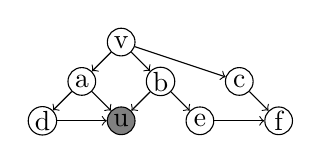
\begin{tikzpicture}[baseline=0pt]
			\begin{scope}[every node/.style={circle,draw,inner sep=0.5pt,minimum size=10pt}, treenode/.style = {circle,draw,inner sep=0.5pt,minimum size=10pt,fill=gray}]
			    \node (d) at (0,0) {d};
			    \node [treenode] (u) at (1,0) {u};
			    \node (e) at (2, 0) {e};
			    \node (f) at (3,0) {f};
			     \node (a) at (0.5, 0.5) {a};
			    \node (b) at (1.5, 0.5) {b};
			    \node (c) at (2.5, 0.5) {c};
			    \node (v) at (1, 1) {v};
			\end{scope}
			\begin{scope}[
			             every node/.style={fill=black,circle},
			              every edge/.style={draw=black}]
			    \path [->] (v) edge  (a);
			    \path [->] (v) edge  (b);
			    \path [->] (v) edge  (c);
			    \path [->] (a) edge  (d);
			    \path [->] (a) edge  (u);
			    \path [->] (b) edge  (e);
			    \path [->] (b) edge  (u);
			    \path [->] (c) edge  (f);
			    \path [->] (d) edge  (u);
			    \path [->] (e) edge  (f);
			\end{scope}
		\end{tikzpicture}
\end{filecontents*}

\begin{filecontents*}{temp3.tikz}
		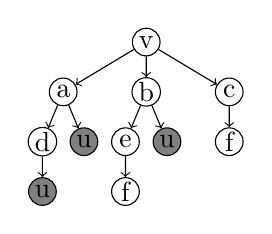
\begin{tikzpicture}[baseline=0pt,->,
		level/.style={sibling distance = 3em/#1,level distance = 1.8em}, 
		interestnode/.style = {circle,draw,fill=gray,inner sep=0.5pt,minimum size=10pt},
		treenode/.style = {circle,draw,inner sep=0.5pt,minimum size=10pt}] 
		\node [treenode] {v}
		    child{ node [treenode] {a} 
		             child{ node [treenode] {d} 
									child{ node [interestnode] {u}}			
		            }
		            child{ node [interestnode] {u}}                    
		    }
		    child{ node [treenode] {b}
		            child{ node [treenode] {e} 
									child{ node [treenode] {f}}			
		            }
		            child{ node [interestnode] {u}}
		    }
		    child{ node [treenode] {c}
		    	  child{ node [treenode] {f} 
		     }
			  }
		; 
		\end{tikzpicture}
\end{filecontents*}

\begin{filecontents*}{temp4.tikz}
  \begin{tikzpicture}[auto, 
%fill=white,
node distance=4cm,
%minimum width=3cm,
font=\small]
  
  
\node[initial,state] (A)                                    {$G_0$};
\node[ellipse (4 and 5), minimum=3cm]         (B) [above right of=A]                 {$G_1$};
\node[ellipse (3 and 2) minimum=2cm]         (C) [below right of=A]                 {$G_2$};
\node[state, minimum=1cm]         (D) [below right of=B]                 {$G_3$};
\node[state]         (E) [above right of=D]                 {$s_4$};
\node[state]         (F) [below right of=D]                 {$s_5$};

 

  \end{tikzpicture}
\end{filecontents*}


\begin{filecontents*}{temp5.tikz}
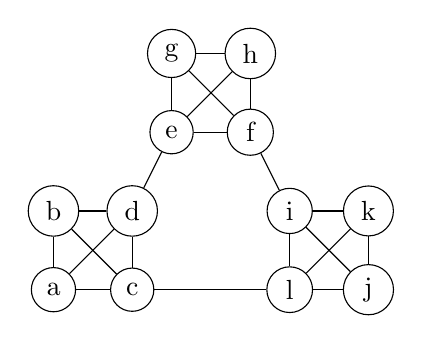
\begin{tikzpicture}
\tikzset{vertex/.style = {shape=circle,draw,minimum size=10 pt}}
\tikzset{edge/.style = {-,> = latex'}}
% vertices
\node[vertex] (a) at  (0,0) {a};
\node[vertex] (b) at  (0,1) {b};
\node[vertex] (c) at  (1,0) {c};
\node[vertex] (d) at  (1,1) {d};

\node[vertex] (i) at  (3,1) {i};
\node[vertex] (j) at  (4,0) {j};
\node[vertex] (k) at  (4,1) {k};
\node[vertex] (l) at  (3,0) {l};

\node[vertex] (e) at  (1.5,2) {e};
\node[vertex] (f) at  (2.5,2) {f};
\node[vertex] (g) at  (1.5,3) {g};
\node[vertex] (h) at  (2.5,3) {h};
%edges
\draw[edge] (b) to (a);
\draw[edge] (b) to (c);
\draw[edge] (a) to (d);
\draw[edge] (b) to (d);
\draw[edge] (c) to (a);
\draw[edge] (c) to (d);

\draw[edge] (e) to (h);
\draw[edge] (e) to (f);
\draw[edge] (e) to (g);
\draw[edge] (f) to (h);
\draw[edge] (f) to (g);
\draw[edge] (g) to (h);

\draw[edge] (i) to (l);
\draw[edge] (i) to (k);
\draw[edge] (i) to (j);
\draw[edge] (l) to (k);
\draw[edge] (l) to (j);
\draw[edge] (j) to (k);


\draw[edge] (f) to (i);
\draw[edge] (d) to (e);
\draw[edge] (c) to (l);
\end{tikzpicture}
\end{filecontents*}

\begin{filecontents*}{temp6.tikz}
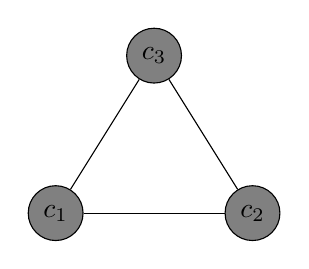
\begin{tikzpicture}
\tikzset{vertex/.style = {shape=circle,draw,minimum size=10 pt, fill=gray}}
\tikzset{edge/.style = {-,> = latex'}}
% vertices
\node[vertex] (a) at  (0,0) {$c_1$};
\node[vertex] (b) at  (2.5,0) {$c_2$};
\node[vertex] (c) at  (1.25,2) {$c_3$};
%edges
\draw[edge] (b) to (a);
\draw[edge] (b) to (c);
\draw[edge] (a) to (c);
\end{tikzpicture}
\end{filecontents*}
%%%%%%%%%%%%%%%%%%%%%%%%%%%%%%%%%%%%%%%%%%%%%%%%%%%%%%%%%%%%%%%%%%%%%%%%%%%%%%%
\begin{document}

%%%%%%%%%%%%%%%%%%%%%%%%%%%%%%%%%%%%%%%%%%%%%%%%%%%%%%%%%%%%%%%%%%%%%%%%%%%%%%%

% 制作国家图书馆封面(博士学位论文才需要)
\makenlctitle
% 制作中文封面
\maketitle
% 制作英文封面
\makeenglishtitle


%%%%%%%%%%%%%%%%%%%%%%%%%%%%%%%%%%%%%%%%%%%%%%%%%%%%%%%%%%%%%%%%%%%%%%%%%%%%%%%
% 开始前言部分
\frontmatter


%%%%%%%%%%%%%%%%%%%%%%%%%%%%%%%%%%%%%%%%%%%%%%%%%%%%%%%%%%%%%%%%%%%%%%%%%%%%%%%
% 论文的中文摘要
\begin{abstract}
在基于图计算的数据分析应用中,如何衡量图中顶点之间的相似度是一个非常重要的问题,在很多领域有重要的应用。
SimRank是近年来比较流行的相似性度量,相比于其他相似度指标,它能更好地反应整个图的结构信息。
然而它的计算代价较高,随着图数据规模越来越大,对SimRank相似度高效的计算方法显得非常必要。
另一方面,Spark作为一种分布式计算平台能够简化用户编写分布式应用的逻辑,自问世以来迅速在学术界和产业界得到广泛的使用。
因此在大数据时代,基于Spark或类似平台设计高效的大规模图数据中点对SimRank相似度的分布式计算方法,有着重要的现实意义。
本文针对上述问题展开了深入的研究,取得的主要成果有:
\begin{enumerate}
 \item 针对图中单源点SimRank相似度计算问题,设计了一种基于随机游走模型的分布式计算方法,并提出了计算过程中的一些优化技巧。
 同时,基于Spark平台给出了算法的分布式实现。
 \item 提出并实现了一种基于模块度优化的多层次分布式图划分方法,算法在划分过程中较好地保留了图中的局部稠密子图,
 在考虑划分约束条件的情况下保证了划分的负载均衡,并力求最小化各个分块之间的边割权重。
 同时,基于Spark平台给出了算法实现。
 \item 基于以上的分布式图划分结果,针对图中全点对SimRank相似度计算问题,设计了一种基于分治思路的近似计算方法。
 该算法通过分别计算分块内点对的相似度以及分块本身的相似度,来估计所有点对的全局相似度。
 算法极大地加速了计算时间,同时结算结果拥有较高的精确度。
 同时,基于Spark平台给出了算法的分布式实现。
\end{enumerate}

% 中文关键词。关键词之间用中文全角分号隔开,末尾无标点符号。
\keywords{图数据;SimRank相似度;分布式计算;Spark}
\end{abstract}研究机构和商业用户

%%%%%%%%%%%%%%%%%%%%%%%%%%%%%%%%%%%%%%%%%%%%%%%%%%%%%%%%%%%%%%%%%%%%%%%%%%%%%%%
% 论文的英文摘要
\begin{englishabstract}
In graph-based data analysis applications, how to measure similarity between vertices in a graph is a
very important research topic which has a wide range of applications in many fields.
Among them, SimRank is one similarity measure with growing popularity in recent years.
Compared with others, SimRank is able to capture the topology of the entire graph. 
However, computation of SimRank is costly in both time and space.
To deal with the ever growing graph size in the era of Big Data, 
efficient computation methods of SimRank is an urgent demand.
On the other hand, as today's popular big data computing engine, Apache Spark significantly simplifies user's programming logic
with the interface it provides when developing distributed applications. 
Therefore, to design an efficient distributed algorithm to compute SimRank similarity for vertex pair in large-scale graphs
based on Spark or other systems is of great significance.

This article addresses the above problems and our main contributions are summarized as follows:
\begin{enumerate}
 \item To compute the single-source SimRank similarity, we designed an algorithm based on the random-walk model.
 Some practical optimizations techniques are proposed. We managed to implement the algorithm on top of Spark.
 \item We proposed a distributed multi-level  partitioning algorithm based on modularity maximization for large graphs.
 In the processing of partitioning, the local dense subgraphs are well preserved within blocks.
 Load balance is carefully maintained with respect to specific constraints, 
 and efforts are made to minimize the edge cut weights between blocks. 
 An implementation of the algorithm based on Spark is presented.
 \item With the help of the above graph partitioning scheme, we proposed an divide-and-conquer algorithm to 
 compute the all-pair SimRank similarity.
 The algorithm partitions the graph into blocks, obtains similarity of each node-pair within blocks, then treats each 
 block as a new vertex forming a coarsening graph to get the similarity between each block. 
 A global similarity for all vertex pairs is approximated based on these two similarities.
 Experiments show that the accuracy of the algorithm is acceptable when the processing time cost is drastically reduced.
 We also give its implementation based on Spark.
\end{enumerate}

% 英文关键词。关键词之间用英文半角逗号隔开,末尾无符号。
\englishkeywords{Graph Data, SimRank Similarity, Distributed Computing, Spark}
\end{englishabstract}

%%%%%%%%%%%%%%%%%%%%%%%%%%%%%%%%%%%%%%%%%%%%%%%%%%%%%%%%%%%%%%%%%%%%%%%%%%%%%%%
% 论文的前言,应放在目录之前,中英文摘要之后
%

%%%%%%%%%%%%%%%%%%%%%%%%%%%%%%%%%%%%%%%%%%%%%%%%%%%%%%%%%%%%%%%%%%%%%%%%%%%%%%%
% 生成论文目次
\tableofcontents

%%%%%%%%%%%%%%%%%%%%%%%%%%%%%%%%%%%%%%%%%%%%%%%%%%%%%%%%%%%%%%%%%%%%%%%%%%%%%%%
% 生成插图清单。如无需插图清单则可注释掉下述语句。
%\listoffigures

%%%%%%%%%%%%%%%%%%%%%%%%%%%%%%%%%%%%%%%%%%%%%%%%%%%%%%%%%%%%%%%%%%%%%%%%%%%%%%%
% 生成附表清单。如无需附表清单则可注释掉下述语句。
%\listoftables

%%%%%%%%%%%%%%%%%%%%%%%%%%%%%%%%%%%%%%%%%%%%%%%%%%%%%%%%%%%%%%%%%%%%%%%%%%%%%%%
% 开始正文部分
\mainmatter

%%%%%%%%%%%%%%%%%%%%%%%%%%%%%%%%%%%%%%%%%%%%%%%%%%%%%%%%%%%%%%%%%%%%%%%%%%%%%%%
% 学位论文的正文应以《绪论》作为第一章
\chapter{绪论}\label{chapter_introduction}
\section{研究背景与意义}
图(graph)作为一种能够刻画实体之间关系的抽象结构,在很多领域中有着重要的应用。
例如,电子商务中商品与用户之间的交易行为,科研著作中各类论文之间的相互参考引用,
Web中个网页之间的链接,以及社交网络中用户之间的交流传播等等行为,本质上都可以
通过基于图来建模。 从图中挖掘出深层次的信息也成了学术界尤其是产业界的一个重要课题。

相似性度量,即比较不同对象之间的相似度,是一个经典的课题。
在推荐系统【】领域,人们关心哪几类商品一定程度上是相似的;
在信息检索【】领域,人们关心如何从WWW找出相似的网页或文章,并对其聚类;
在实体解析领域,人们关心如何从从复杂网络中推测出不同角色是否在真实世界代表着同一个真实实体。
可以看出,现实生活中对相似度的计算无处不在。

而为了准确度量出“相似性”这一概念,学者们提出了各式各样的相似度指标。
其中,SimRank是近年来比较流行的一种度量图中节点相似性的模型,与传统方法不同的是,
它考虑了整个图的拓扑结构,其基本思想与著名的网页排序算法PageRank【】有相似之处:
如果两个顶点的邻居顶点点非常相似,那么这两个顶点也相似。
SimRank相似度可以通过随机游走模型解释,拥有坚实的理论基础,近年来在很多应用中得到了广泛的应用。

传统的SimRank计算,可以归为三类问题:1)单顶点对(single-pair)的相似度计算;
2)单源点(single-source)的相似度计算; 3)全节点对(all-pair)的相似度计算。
这三个计算任务的复杂度依次增加,由计算图中某一对顶点的相似度,
到图中某顶点到其他所有顶点的相似度,再到计算图中所有顶点对的相似度。
正因为SimRank试图充分利用整个图结构的拓扑信息,它的计算具有较高的时间复杂度和空间复杂度。
然而随着互联网技术的发展,人类已经跨入大数据时代。
社交网络用户呈现出爆发性地增长,电子商务变得日益普及,万维网上网络数据也不断增多,现实生活中图数据的规模越来越大。
传统的SimRank相似度计算方法已经无法适用与大规模的图分析任务。


另一方面,在大数据时代诸如MapReduce、Spark等通用式的分布式计算平台正在日益流行。
这些计算平台充分发挥了分布式集群的威力,使得计算能力在横向上扩展(Scale Out)而不是在纵向上提高(Scale Up),
使得原来难以企及的计算任务变得可能。
基于这些平台,用户可以快速部署出自己的解决方案,使用其提供的编程接口专注于自己的计算任务,
而无需关系分布式平台底层的复杂网络通信、资源分配、资源调度问题。

因此,基于此类分布式计算平台设计出高效的分布式SimRank计算方法,具有现实意义。
目前现有的分布式计算方法主要是基于矩阵计算,而对于顶点数超过百万的大图,
其邻接矩阵的元素规模超过万亿,面对如此庞大的输入规模传统基于矩阵计算的方法根本无法满足需求。
面向日益增长的大规模图数据处理的需求,设计新的分布式SimRank相似度计算方法就显得非常必要。


\section{研究现状}
\subsection{SimRank计算研究现状}

\subsection{图划分研究现状}

\section{技术背景}
\subsection{Spark背景介绍}
Aparch Spark 是由美国UC Berkeley AMP Lab开发的通用分布式计算引擎,
目前它已经成为Apache Software Foundation下以及同类大数据开源项目中最受关注的项目之一。
Spark遵循类似于MapReduce的编程范式,但是在执行效率上,
Spark改进了Hadoop[14]批处理框架在迭代计算与交互式处理方面的不足,引入了RDD(弹性分布式数据集)的概念,
允许将计算的中间结果保存在内存之中而无需写入磁盘,大大改善了迭代计算的效率,应用程序的性能得到数十倍甚至百倍的提升;
在用户易用性上,Spark支持Java, Scala, Python等主流编程语言,提供了更加丰富的编程API;
在通用性上,Spark针对不同的开发需求提供了更高阶的库,包括SQL查询,流式计算,机器学习算法以及图计算等等,
开发者可以根据自己的需要,单独或组合使用这些库来处理复杂的数据分析任务。
目前,Spark已经成长为包含Spark SQL,Spark Streaming, MLlib, GraphX等多个子项目的完善的生态系统。
使用Spark,用户只需调用编程接口来实现自己的数据计算任务,而无需关心数据的具体分布、并行调度策略、集群节点之间的数据传送与错误恢复等复杂的底层细节。
凭借其高效、用户友好、通用的优点,Spark在学术界和工业界得到了广泛的实际应用。
\begin{figure}[htbp]
  \centering
  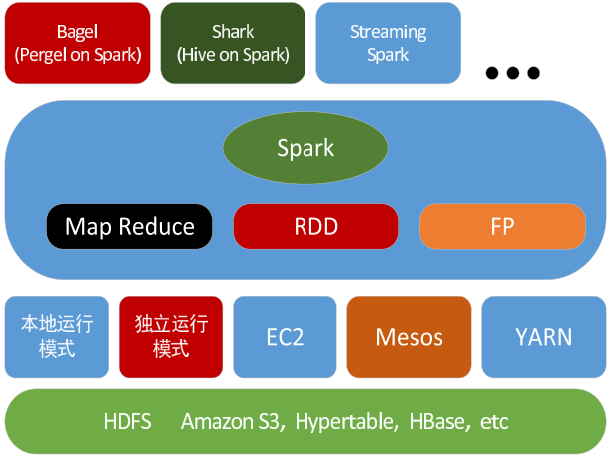
\includegraphics[width= 0.7\textwidth]{figure/spark_stack.png}\\
  \caption{Spark系统架构}\label{fig:spark_stack}
\end{figure}
一个典型的Spark集群通常包括以下几个组件:
1)Driver Program, 每一个Spark应用程序都包含一个driver program,它执行用户的main函数,并负责在集群调度所有的并行化操作。
当应用程序刚从客户端提交上来的时候,Driver Program需要连接到负责分配整个集群上各种资源的Cluster Manager,并向其请求集群上能够使用的Executor。 
然后,Driver Program会把应用程序的Jar包发送给这些Executor,计算过程中会将计算Task分配给这些Executor。
2)Cluster Manager, 它是向集群申请各种资源的一个额外的服务。Spark支持Mesos, YARN等等。
3)Executor, 它是运行在集群中每一个Worker Node上的一个进程,负责本节点上数据的读写以及各种计算。
\begin{figure}[htbp]
  \centering
  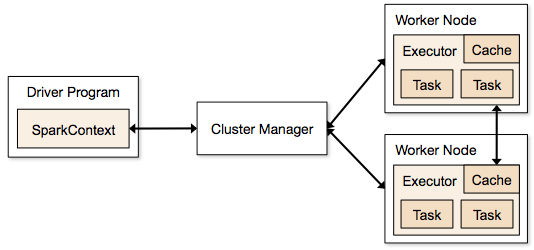
\includegraphics[width= 0.7\textwidth]{figure/spark_components.png}\\
  \caption{Spark系统架构}\label{fig:spark_components}
\end{figure}
%\subsection{Spark数据模型}
Spark采用了一种被称为弹性分布式数据集(RDDs, Resilient Distributed Datasets)的分布式数据抽象,它支持工作集的重用,同时拥有非循环数据流模型(acyclic data flow model)的优点,即数据的负载均衡、位置感知和容错机制。同时RDD是一种受到限制的抽象,这体现在它是只读的,并且只能由已有的分布式数据集或其他RDD执行转换操作来创建。通过递归式地保存自己与其ParentRDD之间的转换记录(lineage),当发生数据分区丢失时RDD可以利用这些记录重新进行计算,快速地恢复数据。
RDD的缺点是它只能提供粒度较粗的转换(coarse-grained transformation)并且它是只读的,这对于一些需要频繁更新数据集的一部分的应用,可能会带来性能上的不足。矩阵计算就是一个需要频繁更新矩阵本身的操作,因此实现算法时要格外注意如何解决这个问题。
RDD可以调用的操作包括转换(transformation)和动作(action)两类。每一个转换操作都会基于调用它的一个或多个parentRdd产生一个新的RDD,所有的转换操作都是懒惰(lazy evaluation)的,这意味着用户在一个RDD上调用一个转换操作并不会立即执行,Spark只是把它当作matadata记住了这些操作。只有当该RDD执行动作操作时,Spark才会利用这些metatada自后往前地追踪到当前RDD最古老的parentRDD,然后从前往后顺序计算这些RDD之间的转换。Spark提供了多种多样的转换,例如map, mapPartitions, union, join, filter等等。
动作(action)指的是需要向driver program返回计算结果或需要将数据导出至存储系统的一类操作。每一个动作都会生成一个Job,对数据进行计算并将计算结果返回给driver。Spark同样提供了多种多样的动作,例如reduce,collect, count, saveAsTextFile等等。
\begin{figure}[htbp]
  \centering
  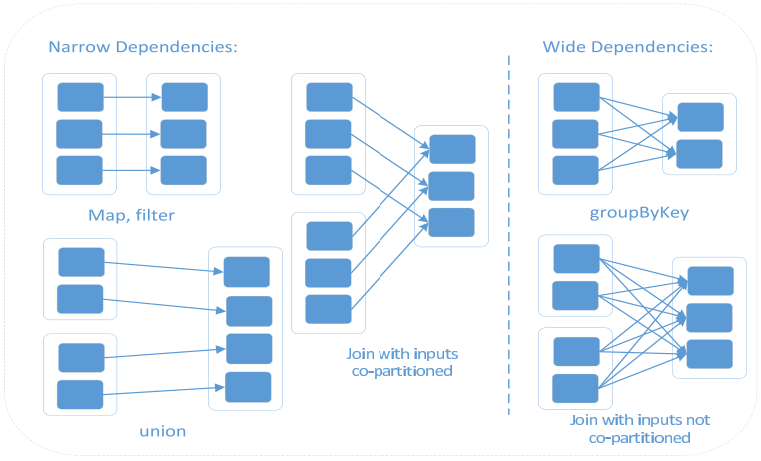
\includegraphics[width= 0.7\textwidth]{figure/rdd_dependency.png}\\
  \caption{Spark系统架构}\label{fig:rdd_dependency}
\end{figure}
%\subsection{Spark常用编程接口}
Spark提供的编程接口,主要包括两类:转化和动作。
其中,典型的转化包括以下几类: 
\begin{enumerate}
 \item {\asciifamily map}一个RDD可以通过map将RDD中的每一个元素通过用户指定的函数转化为另一种类型的元素,
 也就是将原来的RDD转变为指定类型的RDD。map函数接受的参数是一个函数算子。
 \item {\asciifamily mapValues}与map类似,mapValues用于类型为(key, value)的PairRDD。不同的是mapValues不改变元素的key而只改变元素的value,
 因此新的RDD会保留原RDD的partitioner。
 \item {\asciifamily mapPartitions}与map类似,它的第一个参数是一个函数,但mapPartitions是对原RDD的每一个partition而不是每一个element实施这个函数;它的第二个参数是一个Boolen类型,当原RDD的元素类型为(key, value)键值对,并且mapPartitions操作不会改变元素的key时,
 将第二个参数设为true告诉Spark不要改变RDD的partitioner。
\item {\asciifamily filter}一个RDD可以通过filter对RDD中的所有元素按照一定条件进行过滤,过滤后的元素组成一个新的RDD。因此,filter函数接受的参数是一个返回类型为Boolean的函数,这个函数指明一个元素能不能通过筛选。
\item {\asciifamily join}两个元素类型为(key, value)的PairRDD可以通过join操作将双方key相同的元素合并,返回一个新的RDD。
\item {\asciifamily union}两个RDD可以通过union操作合并为一个RDD。
\item {\asciifamily reduceByKey}一个PairRDD调用这个操作可以将原RDD中key相同的若干元素规约为一个元素,返回一个新的RDD。它的第一个参数是一个函数,这个函数相当于元素之间的运算符;第二个可选的参数可以指定新RDD的partition个数。类似于Hadoop中的combiner,spark在shuffle之前会首先对每个计算节点本地的元素先进行合并,从而减小shuffle的开销。
\end{enumerate}
典型的动作包括以下几类:
\begin{enumerate}
 \item {\asciifamily reduce} 它的参数是一个满足交换律、结合律的二元运算符,原RDD的所有元素经过这个运算符计算,返回一个最终值。
 \item {\asciifamily collect} 它将RDD中所有元素从集群上以一个数组的形式返回到Driver Program。collect是一个开销非常大的操作,只适合在小数据集上调用。
\end{enumerate}
还有一种比较特殊的广播操作。通常来说,当集群中的某个节点计算过程中发现需要使用用户自定义的变量时,会向driver program请求将该变量传送到该节点,每一个节点单独地对本地的变量副本进行计算,计算过程中对该副本做出的改动并不会反映到driver program。Spark提供了一种广播变量(broadcast variable), 
它允许开发者主动地将可能在在节点用到的变量广播到集群中的每个节点上,而不用在程序执行过程中当特定节点发现要使用这个变量再从driver program发送到这个节点上。Spark在传送广播变量时使用了一些高效的算法,减少了广播过程中的通信开销。文献[15]表明,在进行迭代计算时,广播变量能极大地提高整体性能。

\subsection{GraphX背景介绍}
GraphX[todo]是Spark生态圈中的一个核心组件, 主要用于图并行计算。
它提供对图计算和图挖掘简洁易用的而丰富的接口,极大的方便了对分布式图处理的需求
GraphX通过引入一个新的图抽象来拓展Spark中的RDD: Resilient Distributed Property Graph,一种点和边都带属性的有向多重图
这里的属性(property)指的是用户自己定义的描述边或定点某些性质的对象。
一个典型的属性图中包含了描述节点信息的VertexRDD和描述边信息的EdgeRDD。
对属性图的所有操作,最终都会转换成其关联的VertexRDD和的EdgeRDD上的相关操作。
这样对一个图计算任务,最终在逻辑上,等价于一系列RDD的转换过程。因此,Graph最终具备了RDD的3个关键特性:Immutable、Distributed和Fault-Tolerant,其中最关键的是Immutable(不变性)。逻辑上,所有图的转换和操作都产生了一个新图;物理上,GraphX会有一定程度的不变顶点和边的复用优化,对用户透明。
\begin{figure}[htbp]
  \centering
  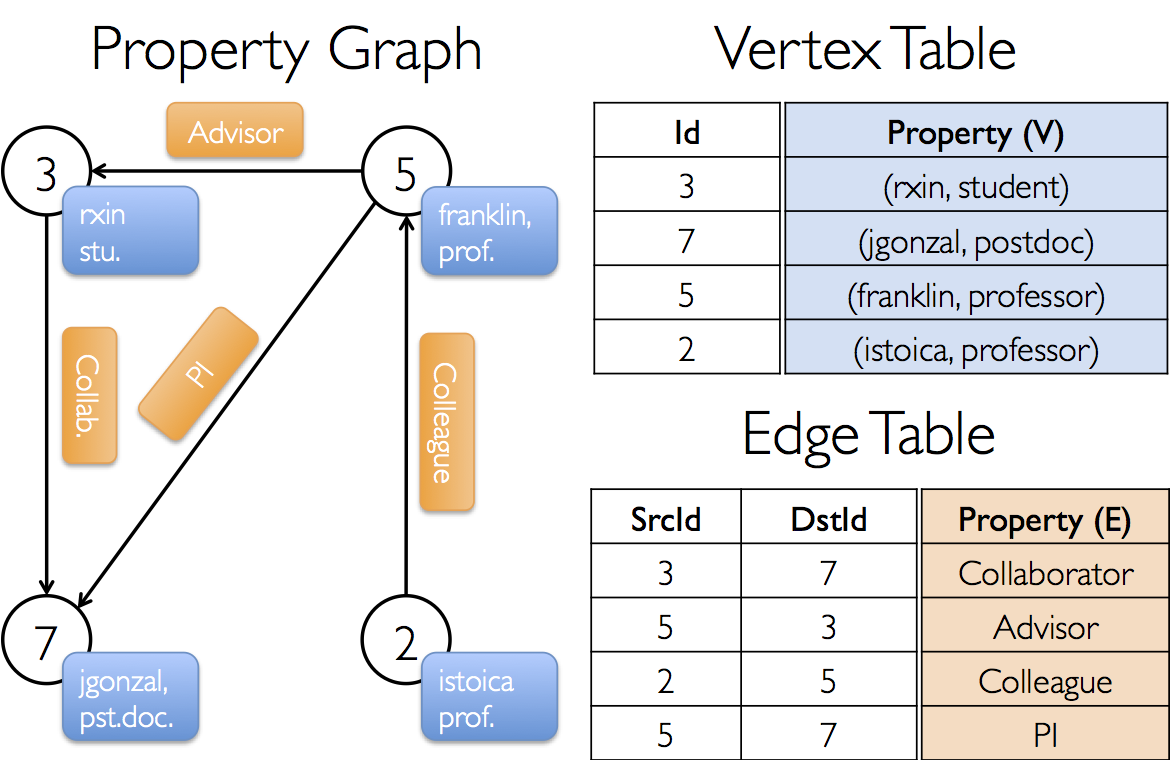
\includegraphics[width= 0.7\textwidth]{figure/property_graph.png}\\
  \caption{一个简单的属性图。左图为图的拓扑信息及其关联的属性;右图为该属性图底层存储的RDD}\label{fig:property_graph}
\end{figure}
%\subsection{GraphX编程范式}

\section{本文主要研究工作}
分析已有的计算方法我们发现,传统的单机SimRank计算方法对于大规模的输入图无能无力,
而现有的分布式算法基本也采用了矩阵计算的思路,而对于一个顶点
数目为百万级别的图,其矩阵的元素基本在万亿级别以上。面对如此大的计算规模,即便分布式处理也无能为力。
在此背景下,本文针对大规模图数据中点对SimRank相似度的分布式计算问题,进行了下列即方面的研究。
本文的创造性研究成果具体如下:
\begin{enumerate}
\item 针对单源点SimRank相似度的计算,提出一种基于随机游走模型的分布式计算方法。
整个算法包含三个步骤:首先生成随机游走,再对游走进行匹配计算其对应概率,
最后汇总得出相似度。
本文设计了一系列优化方法来加速算法过程,包括减少随机游走的数量,使用更紧凑的数据结构来压缩中间数据,以及通过动态规划
的技巧加速随机游走的匹配。本文还对算法的复杂度给出了详尽的分析。

\item 针对大规模图数据,提出一种分布式图划分方法。
该算法能够在保留图中稠密子结构的同时,对图中顶点进行尽量均匀的划分,同时最小化划分之间边的数量(或权重)。
实验表明该分割方法具有较高的效率和划分质量。

\item 基于上诉的图划分方法,进而提出一种计算所有顶点之间SimRank相似度的分布式近似计算方法。
该方法使用分而治之的思想,将所有点对的计算问题划分为若干个子问题,最后再基于子问题的解聚合出初始问题的解。
具体地说,算法首先对图进行划分,然后对每个分块内的顶点对计算局部相似度,然后将各个分块抽象为新的顶点形成一个粗化的图并依次计算各个分块之间的相似度,
最后通过局部相似度和分块相似度共同估算出所有点对的全局相似度。实验表明,我们的方法在大大加速了计算速度的同时,也最大程度地保留了计算结果的准确率。

\item 对上述计算方法,我们分别在流行的通用计算平台Spark上的给出其分布式实现,并使用真实的数据集
在验证算法的精度、效率,以及可扩展性。

\end{enumerate}
\section{论文结构}
本文一共5个章节,每个章节的安排如下:

第一章:绪论。 分别论述了研究背景和意义、研究现状以及现阶段研究尚存在的有待改进的问题、技术背景、本文的主要研究工作和文章总的框架结构。

第二章:分布式单源点SimRank相似度计算方法。 
该章首先对SimRank构建基于随机游走的模型,然后提出算法的框架以及算法中的若干优化思路,接着基于Spark平台实现算法,
最后用实验验证算法各方面的性能。

第三章:分布式图划分方法。该章首先分析了典型的图划分过程的目标和难点,然后对比社区发现与图划分这两个任务的异同,
并提出使用基于模块度的社区发现算法来进行图划分任务。 接着提出算法的主要框架,包括塌缩、初始化分、恢复三个步骤。
我们基于Spark平台给出算法的总体实现,最后通过实验验证算法各方面的性能。

第四章:分布式全点对SimRank相似度计算方法。首先将全点对的相似度计算划分为两个层面的相似度:分块内相似度和分块间相似度。
然后分别给出了这两个相似度的具体计算方法。接着提出了基于上述两个相似度估算全局相似度的方法。
我们基于Spark平台给出算法的总体实现,最后通过实验验证算法各方面的性能。

第五章:总结与展望。总结本文所阐述的所有算法,并对下一步工作做出展望。


%%%%%%%%%%%%%%%%%%%%%%%%%%%%%%%%%%%%%%%%%%%%%%%%%%%%%%%%%%%%%%%%%%%%%%%%%%%%%%%
\chapter{分布式单源点相似度计算方法}\label{chapter_sssSimRank}
\section{概述}
SimRank是一个基于结构上下文的相似度模型,它的核心思想是:如果两个顶点的邻居顶点非常相似,那么这两个顶点也相似。
为了方便描述,首先给出一些通用的符号定义。本文使用关系$(V, E)$表示一个图,其中 $V$是图的顶点集合,
$E \subseteq V \times V$ 是图中边的集合。
$n$ 和 $m$分别是图中顶点的个数、边的个数。顶点$u$ 称作顶点 $v$的入邻点(或出邻点),当且仅当$(u, v)$(或$(v,u)$) 是 $G$中的一条边。
顶点$u$ 的所有入邻点用符号 $I(u)=\{v: (v, u) \in E\}$ 表示,所有出邻点用符号 $O(u)=\{v: (u, v) \in E\}$表示。
图中所有顶点的平均入度(同样也是出度)用符号$d$表示。
顶点$u, v$的间的相似性由$s(u, v)$表示,相应的,所有点对的相似度可以写作 $n\times n$的相似度矩阵$S$,并且有$s(u, v)=s_{uv}$。
顶点$u, v$间的相似值用数学公式如下表达:
\begin{equation}
s(u, v) = \left\{
        \begin{array}{ll}
	1, & \quad u = v ; \\
	\displaystyle\frac{c}{|I(u)||I(v)|}\displaystyle\sum_{u^\prime \in I(u), v^\prime \in I(v)} s(u^\prime, v^\prime), & \quad u \ne v.
        \end{array}
    \right.
	\label{eq:one}
\end{equation}
其中,$0 < c < 1$ 衰减系数,用以提高邻近结构对最终相似性的贡献权重,而降低更远结构的贡献权重。
文献【1】证明了上面的式子总是存在唯一的解,并且基于SimRank的定义,提出了一种基于矩阵乘法的迭代算法。
设 $S^k$是相似度矩阵$S$在第$k$轮迭代中的计算结果,$S^0$为矩阵初始值,并且如果$u = v$ ,有$S_{uv} = 1$,否则$S_{uv} = 0$。
则矩阵$S^{k+1}$的计算方式如下:
\begin{equation}
S^{k+1}_{uv} = \left\{
        \begin{array}{ll}
	1, &\hspace{-0.5em}  \! u = v ; \\
	\displaystyle\frac{c}{|I(u)||I(v)|}\displaystyle\sum_{u^\prime \in I(u), v^\prime \in I(v)} S^{k+1}_{u^\prime v^\prime} , & \hspace{-0.5em} u \ne v.
        \end{array}
    \right.
	\label{eq:two}
\end{equation}
文献【1】已经证明,$\lim_{k\to\infty}S^k_{uv} = s(u,v)$。可以看出,该算法的时间复杂度为$O(n^2)$,空间复杂度为$O(kn^2d^2)$。
\section{相关工作}
为了方便叙述, 我们用$n$表示输入图的节点个数,用$m$表示图的边的个数,用$d$表示图中节点的平均度数。 
对于迭代算法,使用$k$表示算法需要迭代的次数。

\textbf{基于矩阵乘法的计算方法}。 Jeh和Widom提出了第一个基于矩阵乘法的SimRank迭代计算方法,改算法计算全点对的相似性,其复杂度为$O(kn^2d^2)$
.[9]随后通过剪纸、局部访问等技术在矩阵乘法层面将算法的时间复杂度提升到$O(kn^2d)$。【10】使用了快速矩阵乘法来加速计算过程。
文献【12】进一步将算法的时间复杂度提高到$O(kn^2d^{\prime})$,其中$d^\prime < d$。
文献【13】提出了一种基于Keonecker乘积和矩阵奇异值分解(SVD)的非迭代算法,该算法首先在$O(r^4N^2)$时间内计算一些出辅助矩阵,其中$r$是
输入图的领接矩阵的秩,然后再在$O(r^4N^2)$时间内获取给定源点与其他所有节点的相似性。
文献【14】使用了GPU来加速矩阵的计算速度。
对于单点对的SimRank计算,文献【11】给出了一个时间复杂度为$O(kd^2\cdot \min{\{n^2, d^k\}}$的算法。
文献【15】进一步地通过使用概率方法将时间复杂度提高到$O(km^2-m)$。

\textbf{基于随机游走的计算方法}。
图中节点$v$,$u$的相似性,可以解释为:以节点$u$和节点$v$分别为初始点,同步移动的随机游走第一次在某个节点相遇的概率的期望值。
文献【16】给出了第一个基于随机游走的算法, 该算法首先建立一个大小为$O(nN)$的$N$个随机游走的“指纹”索引,然后基于索引查询单点对的相似性。
文献【17】提出一种在随机游走中使用采样技巧计算单点对相似性,该方法在允许一定精度损失的情况下提高了计算效率。
文献【18】研究了图中top-$k$个最相似点对的查询问题,其中$k$往往是一个非常小的值。
该方法把单点对相似查询问题转变为规模为$G\times G$的乘积图上的查询问题。

\textbf{分布式计算方法}。 文献【19】提出了一种基于增量变化的$Delta-SimRank$算法。该算法发现,SimRank可以改写为一种迭代的增量计算方式,
即迭代过程中,不直接改变点对之间的相似性而是计算相对于上一轮迭代的增量。该方法充分利用了迭代计算过程中很多点对间相似性增量为0的事实,减小了
计算过程中的数据传输量。
文献【20】提出了一种基于Spark平台的分布式计算方法,该方法打破了计算点对相似性之间的递归依赖关系:首先线下计算一个不变矩阵$D$,然后线上根据$D$使用
蒙特卡洛方法快速给出查询。然而,$D$的计算被当做一个解线性方程组的过程,这在分布式环境下非常低效,因此虽然算法线上查询的效率很高,
但线下预处理的时间开销非常巨大。

基于以上的SimRank定义以及其基于随机游走模型的解释,计算单源点相似度 $s(u,*)$是非常直接的。
直觉上讲,$s(u,*)$的计算过程可以分解为对$G$中所有节点$v$计算$s(u,v)$的过程。而要计算$s(u,v)$,
我们首先要找出分别从节点$u$和节点$v$出发的所有匹配游走,然后聚合这些游走计算出它们的相遇概率。
注意到想要枚举出任意长度(包括正无穷)的随机游走显然是不可行的,并且显然考虑的长度越长,最后计算得到的相似性越精确。
现实应用中,我们考虑长度为$k$的游走得到的数值可以满足一般应用。
\section{算法基本框架}
\subsection{基于随机游走模型的建模}
SimRank的另一个模型是基于随机游走模型。节点序列$W=v_0v_1v_2\dots v_l$ 如果对任意$0 \leq i \leq l-1$都满足 $(v_i, v_{i+1})$ 都是 $G$ 中的边,
则称其为 $G$中的一个游走。如果$W$还满足以下的Markov条件,即下式对所有的$i \geq1$ ,   $v_0, v_1, \dots, v_i \in V$成立:
\begin{eqnarray}
\label{eq:three}
  Pr(X_i = v_i|X_{0} = v_{0},\dots, X_{i-1}  = v_{i-1}) \nonumber \\  
 =  Pr(X_i = v_i|X_{i-1} = v_{i-1})
\end{eqnarray}
其中,$X_i$ 表示在第$i$部,游走正好到达的节点。
对任意$ u,v \in V$, $Pr(X_i=v|X_{i-1}=u)$表示在第$i-1$步到达节点$u$的随机游走将在第$i$步到达节点$v$的条件概率。
对于SimRank问题,每一条随机游走从某个节点出发,然后顺着图$G$中的逆变,每一个步骤随机走向该节点的某一个入邻点,并且特别的,转移概率定义为
\begin{equation}
Pr(X_i=v_i|X_{i-1}=v_{i-1}) = \left\{
        \begin{array}{ll}
	\frac{1}{|I(v_{i-1})|}, & \quad (v_i, v_{i-1}) \in E; \\
	0,  &\quad otherwise.
        \end{array}
    \right.
	\label{eq:four}
\end{equation}
相应地,一条随机游走的概率,定义为:
 \begin{equation}
Pr(W) = \prod_{i=1}^{l}Pr(X_i=v_i|X_{i-1}=v_{i-1})
	\label{eq:seven}
\end{equation}
现在假设图$G$中有两条随机游走以相同速度分别从节点$u$和节点$v$同时出发,每次都顺着图中的逆边移动,也就是从当前所在节点移动到下一个入邻点,
并且这两条随机游走在同一个节点$x$相遇并且为初次相遇,我们就把这两条终止在节点$x$的游走称作“匹配游走”。
每一对匹配游走的长度就等于随机游走的步骤数。我们基于此定义相遇概率:
 \begin{equation}
Pr\big((W_u, W_v)\big) = Pr(W_u)Pr(W_v)
	\label{eq:five}
\end{equation}
文献【1】表明,节点$u,v$之间的相似度$s(u,v)$等于服从上面概率分布的若干匹配游走的均值:
 \begin{equation}
s(u,v) = \sum\limits_{W_u, W_v} c^lPr\big((W_u, W_v)\big)
	\label{eq:six}
\end{equation}
其中, ($W_u$, $W_v$) 是一对任意的匹配游走,$l$是游走的长度,$c$是前文定义的衰减系数。

文献【11】给出了一个计算单点对SimRank相似度的spSimRank算法。算法的核心思想是两个随机冲浪者分别从节点$u,v$出发,
每一步跟随所在节点的入边;每经过一个节点$t$,原来的随机游走会产生$|I(t)|$ 个新的游走。这样的话经过$k$步游走之后,总共会产生
$O(d^k)$ 个不同的游走,每条随机游走的长度不超过$k$。这些游走使用了一个叫做Path-Tree的数据结构来保存。然后对两个path-Tree中的所有随机游走
进行匹配过程,找出其中的匹配游走。显然与基于矩阵迭代计算的计算方式相比,该算法不需要考虑图中所有的节点。如果我们从这个算法出发,
可以轻易得出一个通过暴力枚举求单源点SimRank相似度的算法。

\begin{figure}
\begin{algorithm}[H]
\captionof{algorithm}{Naive Single-source SimRank:nssSimRank}
\label{algo:nssSimRank}
\begin{algorithmic}[1]
\Procedure{SingleSourceSimRank}{$G, u, k$}
	\For{$ l =1$ to $k$}
		\State $W_u[l] \gets $ all walks of length $l$ starting from $u$;
	\EndFor
	\For {$v \in V(G)$}
		\State $s(u,v)\gets$  \Call{spSimRank}{$G, W_u[], v, k$};
	\EndFor
	\State \textbf{return} $s(u, *)$.
\EndProcedure
\Procedure{spSimRank}{$G, W_u[], v, k$}
\State $s(u, v) \gets 0$;
\For{$ l =1$ to $k$}
	%\State $W_u[l] \gets $ all walks of length $l$ starting from $u$;
	\State $W_v[l] \gets $ all walks of length $l$ starting from $v$;
	\State $s_l(u, v) \gets 0$;
	\For{ $w_u$ in $W_u[l]$}
		\For{ $w_v$ in $W_v[l]$}
		\If {$w_v$ and $w_u$ first meet at index $l$}
			\State add  $score(w_u, w_v)$ to  $s_l(u, v)$;
			\State {\Comment{According to Eq. (\ref{eq:six})}}
		\EndIf
		\EndFor
	\EndFor
	\State add $s_l(u, v)$ to $s(u, v)$;
\EndFor
\State \textbf{return} $s(u, v)$.
\EndProcedure
\end{algorithmic}
\end{algorithm}
\end{figure}
然而,直接通过多次调用spSimRank来计算单源点相似性有以下的缺点:

\begin{enumerate}

\item 总共生成了$O(nd^k)$个游走,但其中大多数的游走都不能匹配到主游走

\item 尽管Path-Tree这种数据结构已经非常高效,但是考虑到会生成$n$个Path-Tree,空间复杂度仍然比较高。
在分布式环境下,因为需要频繁交换节点的局部拓扑信息,这回引起较高的网络开销。

\item 在最后的额匹配过程,统一长度的任意随机游走是以暴力方法匹配的,时间复杂度较高

\end{enumerate}

\section{算法的优化}
\subsection{减少随机游走的数量}
如果直接使用spSimRank算法,总共会生成$O(nd^k)$条随机游走,如果可以将系数$n$减少到某个值$c$使得$C \ll n$,那么游走的数量会极大地减少。
\begin{definition}[倒叙游走]
 我们直接定义随机游走的系列的倒叙序列为倒序游走。
\end{definition}
显然,原始的随机游走与其倒序游走存在一一对应关系。注意到随意游走是在$G$中跟随入边生成的,相应的,倒序游走跟随出边生成。
并且,倒序游走的转移概率需要调整为
\begin{equation}
Pr(X_i=v|X_{i-1}=v_{i-1}) = \left\{
        \begin{array}{ll}
	\frac{1}{|I(v_{i})|}, & \quad (v_{i-1}, v_i) \in E; \\
	0,  &\quad otherwise.
        \end{array}
    \right.
	\label{eq:eight}
\end{equation}

基于倒序游走的定义,可以观察到有下列现象:
\begin{fact}
假设两个分别从节点$u, v$开始的随机游走$W_u, W_v$经过$l$步后在节点$x$相遇,那么如果我们从节点$x$ 出发生成所有长度为$l$的倒序游走,
$W_u, W_v$ 的倒序游走一定也在其中
\end{fact}
\begin{fact}
 假设$W_u=uw_1w_2\dots w_l$是一条主游走,则所有有可能与$W_u$在 $l$步相遇的从游走,只能在$\{w_1, w_2, \dots, w_l\}$中的任意一点相遇。
 也就是说,设$Nei$是节点$u$在$k$部可达的点集,那么只要生成从$Nei$出发的倒序游走就可以计算$s(u,*)$。
\end{fact}

以上两个事实的正确性是显然的。可以看出,总共需要生成的倒序游走的数量大约在$O(|Nei|d^k)$而不是暴力算法的$O(nd^k)$。
事实上, $|Nei|$ 的复杂度为$O(d^k)$, 远比图$G$中点数目小,并且独立于$G$真实大小。

\begin{figure}[t]
\centering
\label{fig:graph1}
\resizebox{!}{!}{\begin{tikzpicture}
    \matrix(dict)[matrix of nodes, %below=of game,
        nodes={align=center,text width=20em,text height=5em},
        %row 3/.style={nodes={text height =1em}},
        %column 1/.style={nodes={text width=10cm,align=right}}
    ]{
        $u, w_1, w_2, w_3, \dots, {x}, \dots$ & $x, \dots, w_3, w_2, w_1, u, \dots$ \\
       $v, w^\prime_1, w^\prime_2, w^\prime_3, \dots,{x}, \dots$  & $x, \dots, w^\prime_3, w^\prime_2, w^\prime_1, v, \dots$ \\
       %(a): walk starting from u and v & (b) reversed walks starting from x \\
       %(a) & (b) \\
    };
\end{tikzpicture}
}
\caption{The left are two walks starting from $u$ and $v$ respectively, first meeting at $x$; the right are reversed walks starting from $x$, passing $u$ and $v$ respectively.}\label{fig:one}
\end{figure}


\begin{figure}[t]
    \centering
    %\subfig[fjalkf]
    \begin{subfigure}[b]{0.48\linewidth}        %% or \columnwidth
        \centering
        \label{fig:match_walks_one}
	\resizebox{!}{!}{  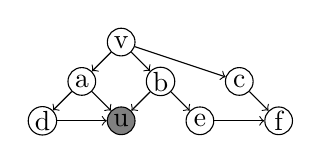
\begin{tikzpicture}[baseline=0pt]
   \begin{scope}[every node/.style={circle,draw,inner sep=0.5pt,minimum size=10pt}, treenode/.style = {circle,draw,inner sep=0.5pt,minimum size=10pt,fill=gray}]
       \node (d) at (0,0) {d};
       \node [treenode] (u) at (1,0) {u};
       \node (e) at (2, 0) {e};
       \node (f) at (3,0) {f};
        \node (a) at (0.5, 0.5) {a};
       \node (b) at (1.5, 0.5) {b};
       \node (c) at (2.5, 0.5) {c};
       \node (v) at (1, 1) {v};
   \end{scope}
   \begin{scope}[
                every node/.style={fill=black,circle},
                 every edge/.style={draw=black}]
       \path [->] (v) edge  (a);
       \path [->] (v) edge  (b);
       \path [->] (v) edge  (c);
       \path [->] (a) edge  (d);
       \path [->] (a) edge  (u);
       \path [->] (b) edge  (e);
       \path [->] (b) edge  (u);
       \path [->] (c) edge  (f);
       \path [->] (d) edge  (u);
       \path [->] (e) edge  (f);
   \end{scope}
  \end{tikzpicture}
}
	\caption{$N_G(v, 4)$.}
	
	\end{subfigure}
    \begin{subfigure}[b]{0.48\linewidth}        %% or \columnwidth
     \centering
	\resizebox{!}{!}{  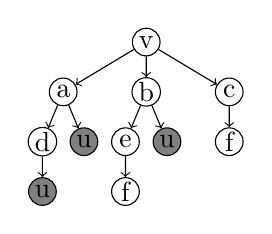
\begin{tikzpicture}[baseline=0pt,->,
  level/.style={sibling distance = 3em/#1,level distance = 1.8em},
  interestnode/.style = {circle,draw,fill=gray,inner sep=0.5pt,minimum size=10pt},
  treenode/.style = {circle,draw,inner sep=0.5pt,minimum size=10pt}]
  \node [treenode] {v}
      child{ node [treenode] {a}
               child{ node [treenode] {d}
         child{ node [interestnode] {u}}
              }
              child{ node [interestnode] {u}}
      }
      child{ node [treenode] {b}
              child{ node [treenode] {e}
         child{ node [treenode] {f}}
              }
              child{ node [interestnode] {u}}
      }
      child{ node [treenode] {c}
         child{ node [treenode] {f}
       }
     }
  ;
  \end{tikzpicture}
}
	\caption{Path-tree of $N_G(v, 4)$.}
	\label{fig:match_walks_two}
    \end{subfigure}
    \caption{(a) A neighborhood of $v $.  (b) The corresponding Path-Tree representation of the neighborhood.}
    \label{fig:match_walks}
\end{figure}

\subsection{压缩中间数据的表示}
相比于尽管生成游走的减少了很多,但是$O(d^k)$复杂度依旧很高。
而这些游走序列之间会有很多前缀子序列高度重合,如果单独地保存每一条游走,那么整个存储会有较大的冗余。
TODO
为了解决多个游走序列共享很多前缀子序列,对$|Nei|$中的每一个节点$v$,我们并不使用任何特别设计的数据结构单独存储从$v$的所有随机游走,
而是直接使用从$v$开始跟随逆边$k$可达的一个邻域$N_{G}(v, k)$。
严格的说,$N_{G}(v, k)$是节点从$v$跟随逆边$k$步可达的节点集合在$G$中的生成子图。
例如,在图【4】中,展示了$v$的一个邻域。他所对应的path-tree显示在右图中,灰色的节点是我们欲查询的节点$u$。
可以看到,$N_{G}(v, k)$自己本身就是Path-Tree的一种压缩表示。
显然,我们在这一步中没有显式地表示出每一条游走,是因为在分布式环境中生成游走的过程需要在不同的计算节点上传输$G$中的局部拓扑信息,
如果中间传输数据量过大,那么网络开销会极大地影响算法的最终性能。我们在下面会详细叙述即使没有显式表示每一条游走,算法仍然可以高效地计算出最终结果。

\subsection{使用动态规划技巧加速随机游走的匹配}
当$Nei$中的每个节点$v$收集到了从它自己开始的倒序游走$N_{G}(v, k)$之后,这些从游走需要与主随机游走$N_{G}(u, k)$进行匹配,从而得到最后的结果。
由于代表所有主游走的$N_{G}(u, k)$只是一个很小的信息($O(d^k)$),我们可以把它预先广播到分布式集群中的每一个节点上。
而所有的从游走$N_{G}(v, k)$按照$v$作为key分不到不同的节点上,然后每个计算节点直接在本地进行匹配过程。
正因为这样,算法中最耗时的匹配部分是分布到每个计算节点上进行的,这是我们设计该算法的主要目的。

为了方便叙述,我们以在节点$v$第一次相遇的随机游走为例。
注意整个匹配过程中,我们只对与主游走在$v$相遇,但是之后再也不和主游走有任何共同节点的逆序游走感兴趣。
例如,在\ref{fig:match_walks_two}中,路径$vau$和$vbe$是一对对$s(u,e)$有意义的匹配游走。
同理,和$vau$能匹配上的随机游走还包括$vau$和$vcf$。
但是,$vad$和$vau$不是一对合法的匹配游走,因为它们首次在节点$a$而不是$v$首次相遇。实际上,
$vad$和$vau$同样对$s(d,u)$的计算做出了贡献,但是在分布式环境下,这个计算过程是由形如图\ref{fig:match_walks_two}、但root
节点为$a$的Path-Tree引导的。这个计算过程也应当发生在该Path-Tree的计算节点上。
基于以上的简单观察,可以发现以下事实:
\begin{fact}
如果我们的查询节点$u$处于某个Path-Tree的某一层里,那么那一层的其他任一满足$LCA(u, w)=v$的节点$w$都会对节点$u,w$的相似度$s(u,w)$的计算做出
大小为$c^{l}Pr(W_u)Pr(W_w)$的贡献,其中$LCA$指的是最近公共祖先(Lowest Common Ancestor),
$W_u, W_w$是由对应Path-Tree展开的root-to-node路径。
\end{fact}
我们使用DFS算法来搜索整个领域$Nei_v$。 
在DFS过程中,每一条root-to-node路径的概率被记录下来。
当DFS的深度达到$l$时,算法停止,对应逆序游走的概率被保存在一个HashMap中。
当我们再次匹配长度为$l+1$的主游走时,就不再需要从节点$v$开始我们的DFS过程,因为该Path-Tree中长度小于等于$l$的逆序游走的概率之前已经全部计算过了。
例如,在图\ref{fig:match_walks_two}中,能和游走$vbdu$匹配的唯一游走是$vbef$,而计算$vbef$的概率时,我们只需要从节点$e$开始DFS过程,
因为$vbe$的概率在之前搜索$vae$的匹配游走时已经计算被保存过了。

因此为了克服多个游走之间共享了很多重复前缀这一问题,我们把匹配游走这一问题看做是一个动态规划(Dynamic Programming)问题,
通过Memorization的技巧来降低匹配的时间复杂度。算法的具体细节在\ref{alg:dp}中列出。
程序LevelMatch展示了一个Path-Tree中的根节点$v$如何寻找一个长度为$l$的主游走。
各参数的意义如下:$W_l$是长度为$l$的主游走的集合;$N$是从节点$v$开始展开的领域;$M_{l^\prime}$ 
保存了之前调用LevelMatch函数来匹配长度为$l^\prime$主游走得到的匹配概率,具体地说它是一个(key,value)形式的HashMap,
其中key是$v$的邻居节点,表示该k-v对保存的是以Path-Tree中第二层节点为根节点的哪一棵子树的信息,
value是一串元素,每个元素记录着以$key$为根节点的子树中所有的游走的终止节点以及对应游走的概率;
类似的$M_l$是一个将要被填充的空的HashMap,保存匹配长度为$l$的游走的匹配概率;
最后一个参数$\delta$是一个概率阈值,其具体的含义将在下一节给出。
我们首先循环$W_l$中的每一条主游走$p$,并且知道该主游走在Path-Tree中的哪一棵子树中(2-3行),如果$M_l$中没有记录该子树中匹配游走的概率,
就开始DFS过程(4行)。
我们先检查$W_{l\prime}$中是否有记录该子树的信息,如果有的话就直接从记录的游走的终止节点开始调用DFS(5-6行),
否则就需要从该子树的根节点开始DFS。
程序DFS就是一个常见的DFS过程。
通过对所有的$W_l, (l \leq k)$,所有游走的匹配概率都可以高效地计算出来。


\begin{figure}
\begin{algorithm}[H]
\captionof{algorithm}{Dynamic Programming Path Matching}
\label{alg:dp}
\begin{algorithmic}[1]
\Procedure{LevelMatch}{$W_l, N, v, M_{l^\prime}, M_l, \delta$}
	\For {$p \in W_l$}
		\State {$br \gets$ second last vertex of $p$};
			\For {$t \in (v_N.neighbors - br)$ \& $t \notin M_l$}
				
					\If {$!M_{l^\prime}$.contains$(t)$}
						\State \parbox[t]{\dimexpr\linewidth-\algorithmicindent} {\Call{DFS}{$N, t, l, M_l,\delta, t, 1, 1$};}	
					\Else 
						\For {$w \in M_{l^\prime}$}
							\For {$nei \in w_N.neighbors$}
								\State \parbox[t]{\dimexpr\linewidth-\algorithmicindent}{\Call{DFS}{$N, nei, l,M_l,\delta,br,w.mul, l^\prime$};}
							\EndFor
						\EndFor
					\EndIf			
				
			\EndFor
	\EndFor
	\State \textbf{return} $M_l$.
	%\State \textbf{return} $results$.
\EndProcedure
\Procedure{DFS}{$N, v, l, M,\delta ,br ,mul,depth$}
	\State {$mul \gets mul * v_N.indegree$};
	\If {$mul > \delta$}
		\State \textbf{return;} \Comment{Early termination.}
	\EndIf
	\If {$depth = l$}
		\State {add $(v, mul)$ to $M(br)$};  \Comment{Record  probability.} %to the branch it resides in.}
	\Else
		\For {$nei \in v_N.neighbors$}
			\State \parbox[t]{\dimexpr\linewidth-\algorithmicindent} {\Call{DFS}{$N, nei, l, M,\delta, br,mul$, $ depth+1$};}
		\EndFor
	\EndIf
	\State \textbf{return} $M$.
\EndProcedure
\end{algorithmic}
\end{algorithm}
\end{figure}
\subsection{使用概率阈值剔除极小的概率}
很多现实的大图都是scale-free【21】的,这意味这图中的极小比例的节点会有极高的度数。
我们的算法的性能与节点的度数紧密相关,因为在生产游走过程中每条游走每经过一个度数为$d$的节点,都会在那个节点分裂为$d$条更长的游走。
因此,我们使用一个阈值$\delta$来删除那些包含多个拥有极高度数的节点的游走,因为根据公式【TODO】,这些游走对的概率非常之小,
对最终的计算精度基本可以忽略不计。$\delta$的取值应当注意在算法的精度与时间、空间复杂度取得平衡,更大的$\delta$意味着更低的精度,当时算法
整体的时间复杂度和空间复杂度更低,反之反是。
\section{算法的复杂度分析}
我们综合分析一下算法的复杂度。源点$u$可达的节点的数目大约为$O(d^k)$,
而对于其中的每一个可达节点,都拥有一个大小为$O(d^k)$,隐式包含$O(d^k)$条逆序游走信息的领域,
因此,总的空间复杂度为$O(d^{2k})$。因为这个过程中所有产生的游走都需要通过网络传输,所以通信开销也是$O(d^{2k})$。
在对游走进行匹配时,对每一个领域,大约有$O(d^k)$个游走被匹配了,所以总的计算复杂度为$O(d^{2k})$。
可以看到,算法总的复杂度与整个图的规模$O(n+m)$没有以来关系,所以我们的算法是非常高效的。
\section{基于Spark平台的算法实现}
基于Spark平台的算法实现可以概括为4个步骤:
\begin{enumerate}
 \item 找出从顶点$u$出发顺着入边经过$k$部可达的邻域$Nei$,同时记录所有的主游走。然后将所有的主游走广播到集群所有计算节点上。
 \item 从$Nei$中每一个顶点$v$出发,顺着出边找出其$k$步可达的邻域,这些邻域看做一个以$v$为key的key-value对,散布在集群中。
 \item 对上面每一个$v$的邻域,和第一步中的$Nei$进行匹配,计算匹配概率。
 \item 聚合所有的匹配概率得出最终的相似度$s(u,*)$。
\end{enumerate}
上述四个步骤中第1个和第2个很相似,区别只是要获得邻域的顶点的数量(1 vs $|Nei|$)。
因此我们重点描述第2、 3、 4步骤在Spark平台上的实现。
\subsection{邻域收集步骤}
代码\ref{algo:nei_collect}展示了生成邻域的具体细节。
算法总共接受3个参数:$edgeRDD$表示从HDFS读入的、每个元素代表图中一条边的RDD,$Nei$是要生成邻域的出发顶点集合,$k$是游走的最大长度。
首先我们把图从按照边存储的格式变为邻接表这种格式,并存储在$graphRDD$中(第2-3行),
然后我们从$graphRDD$生成$nbrhdRDD$(第4行),这个RDD里面存放着所有的邻域。
$nbrRDD$表示所有邻域的最外面一层,初始化时它就是集合$Nei$的直接邻居顶点(第5行)。
接下来算法以迭代方法不断纳入新的边对$nbrhdRDD$进行扩张,即把之前邻域最外围的顶点$nbrRDD$的邻居节点纳入到邻域中。
每一次扩张也代表着游走的最大长度增加了一步,这个操作是通过Spark中的连接(join)操作完成的。
每次扩张时通过$nbrRDD$与$graphRDD$做连接操作得到最新的最外围顶点(第7-8行),
再通过$nbrhdRDD$与$nbrRDD$做连接操作把这些顶点纳入到邻域中(第9-10行)。
\begin{algorithm}[H]
\captionof{algorithm}{Collect Neighborhood}
\label{algo:nei_collect}
\begin{algorithmic}[1]
	\Procedure{Collect}{$edgeRDD, Nei, k$}
		\State {$graphRDD \gets edgeRDD$}
		\State {\qquad .{\asciifamily reduceByKey}$()$.{\asciifamily cache}$()$};
		\State {$nbrhdRDD \gets graphRDD$.{\asciifamily map}$()$.{\asciifamily cache}$()$};
		\State {$nbrRDD \gets graphRDD$.{\asciifamily filter}$()$.{\asciifamily cache}$()$};
		\For{$ l =2$ to $k$}
			\State {$nbrRDD \gets  nbrRDD$}
			\State {\qquad.{\asciifamily join}$(graphRDD)$.{\asciifamily map}$()$};
			\State {$nbrhdRDD \gets nbrhdRDD$}
			\State {\qquad .{\asciifamily leftOuterJoin}$(nbrRDD)$.{\asciifamily map}$()$};
		\EndFor
	\State \textbf{return} $nbrhdRDD$.
	\EndProcedure
\end{algorithmic}
\end{algorithm}
\subsection{匹配游走步骤}
当所有邻域全部生成完毕后,我们开始匹配主游走和从游走。具体细节如算法\ref{algo:match}所示。
程序接受4个参数:$nbrhdRDD$表示程序\ref{algo:nei_collect}的返回结果;$MW$表示被广播到集群各个计算节点上的所有主游走,
其数据结构是一个由$key-value$对组成的HashMap,其中$key$是每个主游走的终止顶点(因此$key \in Nei$),
$value$是所有以$key$终点的随机游走;剩下两个参数$u$和$k$分别是查询节点和游走的最大长度。
对$nbrhdRDD$中的每个元素$(v,nbrhd)$,我们调用算法\ref{alg:dp}计算$nbrhd$中所有游走的匹配概率。
注意到$nbrhdRDD$中的所有元素以$v$为$key$被Spark默认的Partitioner均匀分布在集群中,因此整个计算过程是分布式的。
计算出的结果被组装成一个列表(第7行),然后经flagmap操作发射出去(第8-9行),
最后经由reduceByKey操作将属于不同$v$的相似度$s(u,v)$聚集起来,并送至Driver Program(第11-12行)。


\begin{algorithm}[H]
\captionof{algorithm}{Compute SimRank}
\label{algo:match}
\begin{algorithmic}[1]
\Procedure{Compute}{$nbrhdRDD, MW,  u, k$}
	\State {$simRankRDD \gets hbrhdRDD$}
	\State {\qquad .{\asciifamily flatMap}$((v, nbrhd) \Rightarrow\{$}
	\State {\qquad \qquad create $MP$};
	\State {\qquad \qquad \textbf{for} $W_l$ in $MW$ \textbf{do}}
	\State {\qquad \qquad \qquad $M \gets$ \Call{LevelMatch}{$W_l, \dots $}};
	\State {\qquad \qquad \qquad extend $MP$ with all elemetns in $M$};
	\State {\qquad \qquad \textbf{for} $(v, score(u,v))$ in $MP$ \textbf{do}}
	\State {\qquad \qquad \qquad yield $(v, score(u,v))$};
	\State {\qquad $\})$}
	\State {$s(u,*) \gets simRankRDD$.{\asciifamily reduceByKey}$()$.{\asciifamily collect}$()$};
	\State \textbf{return} $s(u, *)$.
\EndProcedure
\end{algorithmic}
\end{algorithm}


\section{实验评估}
\subsection{实验环境}
所有的实验在一个由6个硬件完全相同的计算节点组成的集群上完成,每台计算节点处理器为12核的Intel Xeon E-2650,频率为2.1GHz,
内存为64GB,硬盘为1TB。 计算节点之间由千兆网卡连接。所有的节点上运行Ubuntu 16.04操作系统。 
Spark运行版本为1.6.2, 底层分布式文件系统HDFS的版本号为2.6.0。
所有的6个节点都配置为slave节点,其中一个节点被二外配置为master节点。 
在Spark运行时,我们为其分配了10GB的内存。
\subsection{实验数据集}
我们一共使用了5个真实的图数据来评估算法的性能。 数据集的具体细节如表\ref{tab:dataset1}。
每个图一开始为普通的文本形式,每一行代表这图中的一条边。
在开始实验前,所有的数据集都预先上传到分布式文件系统HDFS上。
\begin{table}[h]
\caption{数据集描述}
\label{tab:dataset1}
\centering
\begin{tabular}{|l|r|r|r|r|}
\hline
\textbf{数据集} & \textbf{顶点数} & \textbf{边数} & \textbf{顶点平均度数} & \textbf{大小} \\
\hline
p2p-gnutella08 \footnotemark[1]  & {6,301}         & \num{20777}                   & 3.29                & 215.2KB\\
\hline
wiki-vote \footnotemark[2]    & 7,115 	& \num{103,689}                           &14.57                & 1.1MB  \\
\hline
%wiki-talk            & \num{2394385} & \num{5021410}          &2.10                   & 66.5MB\\
%\hline
eu-2005       \footnotemark[3]     & \num{862664}  & \num{19235140 }          & 22.29             & 256.4MB\\
\hline
ljournal-2008  \footnotemark[4] & \num{5363260} & \num{79023142}         & 14.73            &1.2GB\\
\hline
arabic-2005 \footnotemark[5]   & \num{22744080} & \num{639999458}      & 28.14           & 10.9GB\\
%\hline
%twitter-2010    & \num{41652230 } & \num{1468365182} & 26.1GB\\
\hline
\end{tabular}
\end{table}
\subsection{实验参数设置}
根据文献文献【9】中的描述,通常算法所需要的最大迭代次数$k$是由衰减系数$c$和算法的预期精度决定的。 
如果希望最终误差 $s^*(u,v) - s^k(u,v)$小于某个$\epsilon$,那么$k$至少要被设置为$k=\lfloor \log_c \epsilon \rfloor$。
在我们的实验中,我们选取$\epsilon=0.01$,因为这样的精度可以满足大多数实际应用。 
$c$被设置为0.5,相应的,$k$被设置为$k=6$。

此外,用于过滤掉极小概率的游走的阈值被设置为$\delta=0.002$。主要到这里的$\delta$指的是一个随机游走的概率阈值,
根据\ref{eq:five}对于一对匹配好的游走,其对应的匹配概率相应的变成${\delta}^2$。
如果再考虑到因子$c^l$,那么这个概率是极端小的,完全可以忽略。

算法精度的测试采用的方法是多次实验取平均值,每次实验时随机选取图中的某个顶点为查询顶点。
具体的,对与小图(大小<10MB),我们重复实验100次计算其平均值;对于更大的图,重复次数设为1000。
\subsection{算法有效性}
\begin{figure*}[t]
\centering
\begin{subfigure}[b]{0.48\textwidth}
	\center
	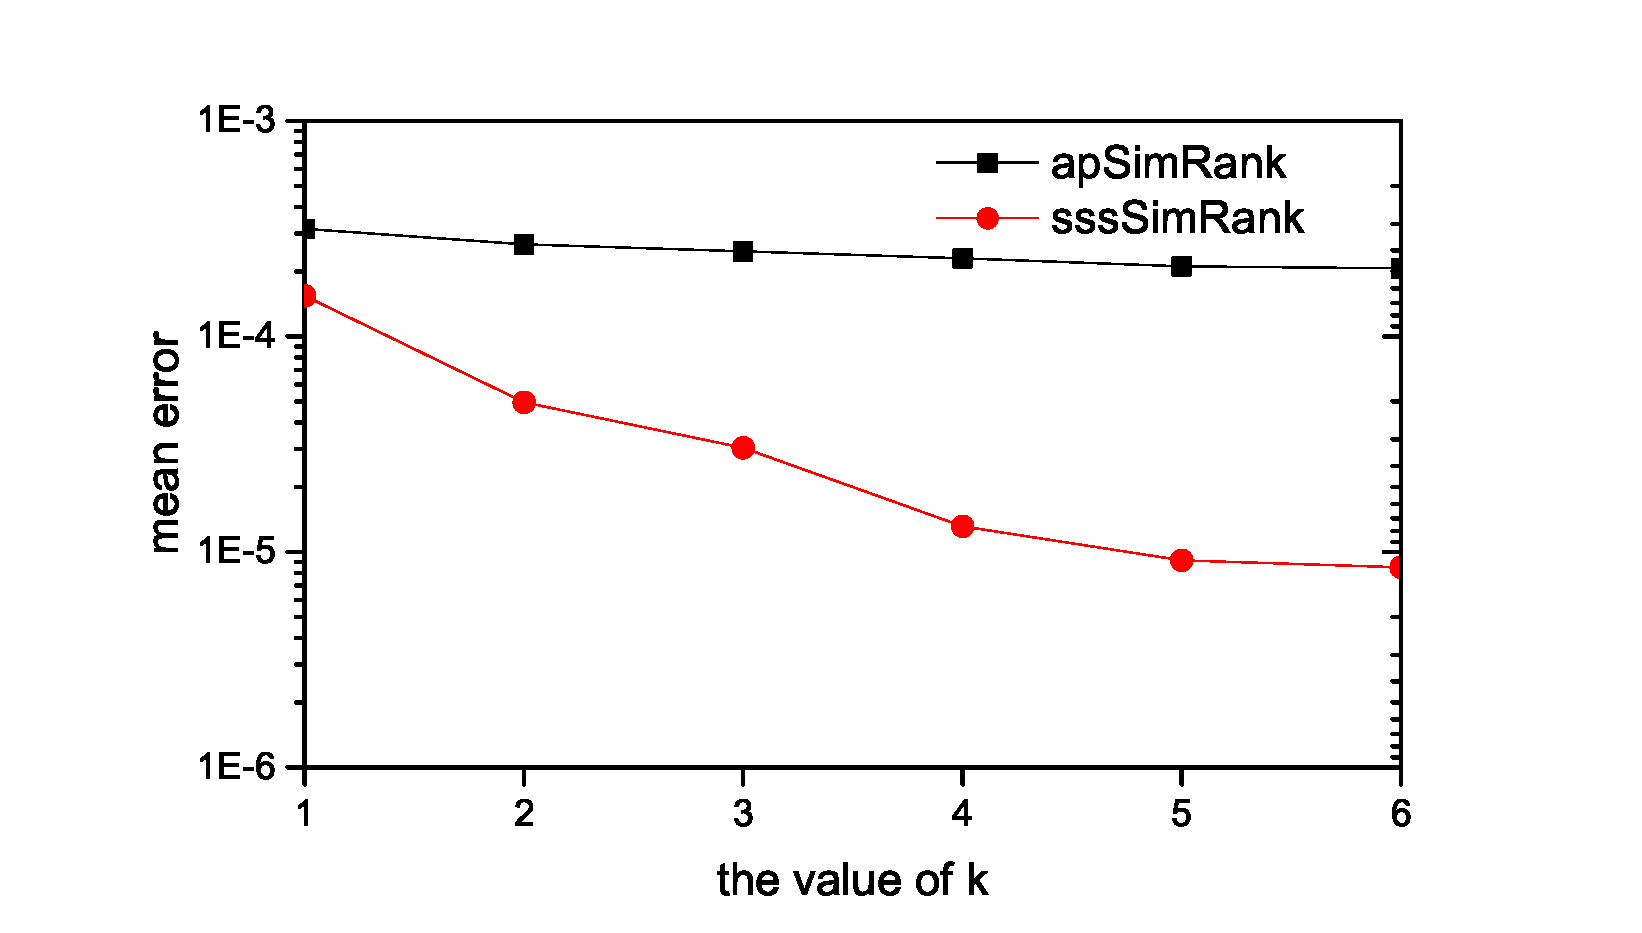
\includegraphics[width=1\textwidth]{figure/accuracy1.eps}
	\caption{p2p-gnutella08}
	\label{fig:ch1:effec:one}
\end{subfigure}
\begin{subfigure}[b]{0.48\textwidth}
	\centering
	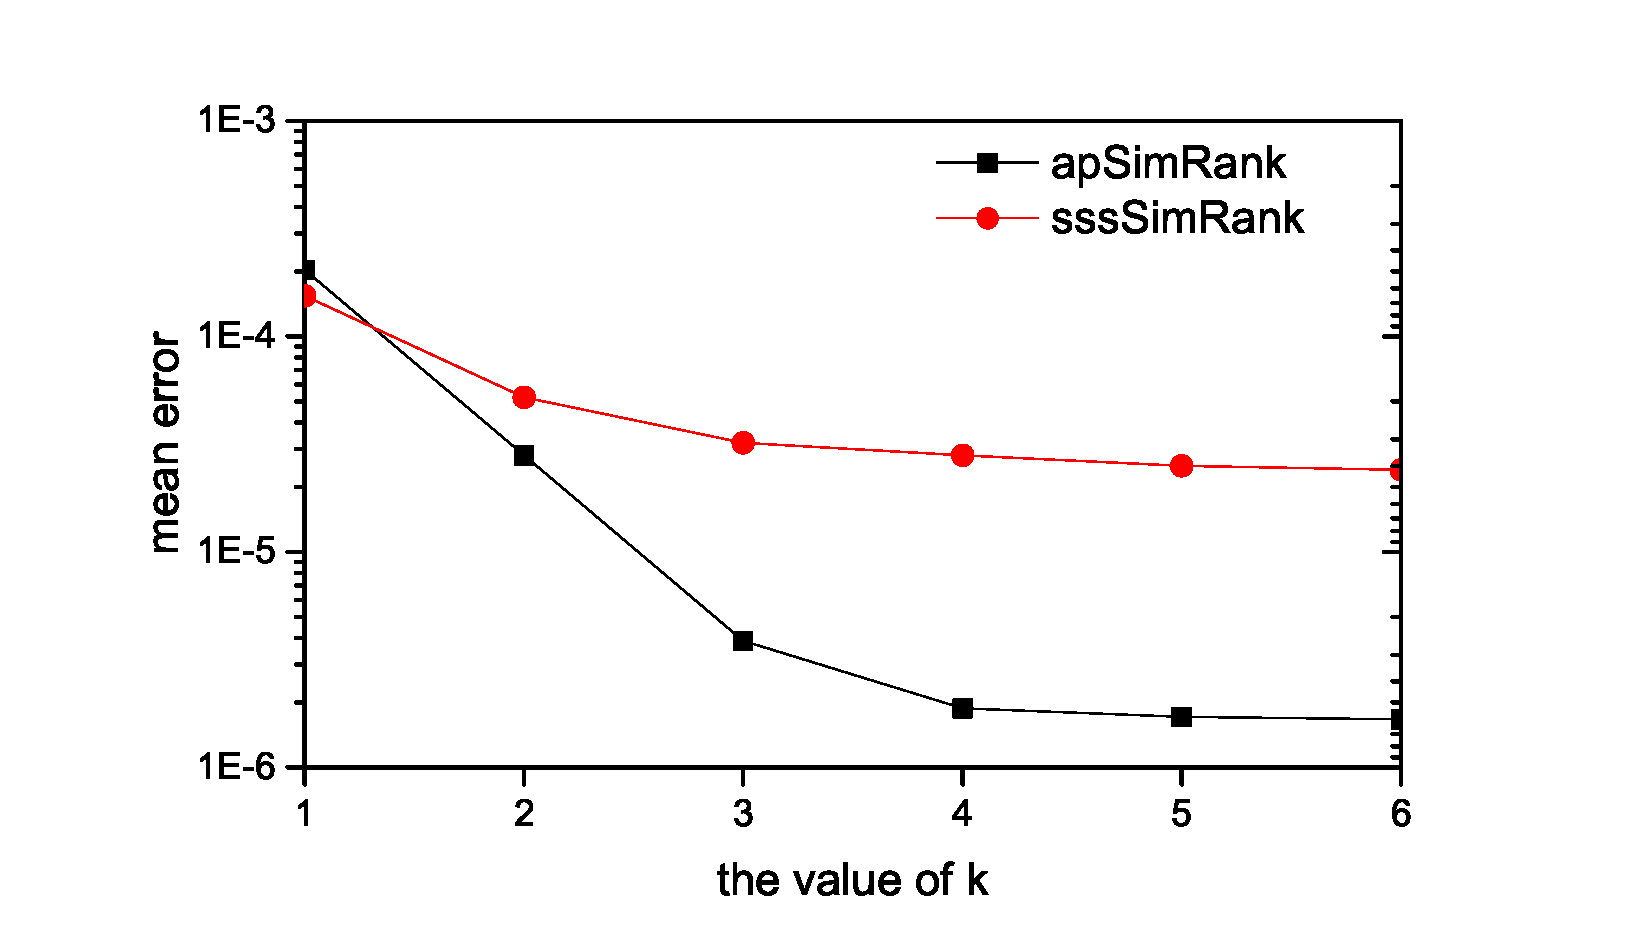
\includegraphics[width=1\textwidth]{figure/accuracy2.eps}
	\caption{wiki-vote}
	\label{fig:ch1:effec:two}
\end{subfigure}
\label{fig:ch1:effec}
\caption{apSimRank和sssSimRank的相似性误差随迭代次数的变化曲线比较}
\end{figure*}
我们首先比较我们的算法和全点对算法的精度和收敛速度。
我们选取的精度指标为平均误差(mean error),即$ME = \frac{1}{n}\sum_{v \in V}{\left|s(u,v) - s^k(u,v)\right|}$,
其中$s(u,v)$为根据\ref{eq:two}迭代计算至完全收敛的真实相似性,$s^k(u,v)$为我们算法迭代$k$次后的相似性。
我们在两个小图上进行实验。其中p2p-gnutella08是个比
较稀疏的图,平均顶点度数$d=3.29$,而wiki-vote是一个更加稠密的图,平均顶点度数为$d=15.57$。
图\ref{fig:ch1:effec}为最终的比较结果。
从图中可以看到,全点对算法和我们的算法在6次迭代以内精度都得到了收敛, 我们的算法sssSimRank有更好的收敛速度,三次迭代之后平均误差就在$10^{-4}$以内。
另一个现象是在图\ref{fig:ch1:effec:one}中sssSimRank的平均误差与apSimRnak的差距比图\ref{fig:ch1:effec:two}更小,
这是因为我们的算法中使用了概率筛除的缘故。对于同一个概率阈值$\delta$,图的平均顶点度数越大,小概率游走越多, 相应的,被剔除的小概率游走越多,
所以对最终精度的影响越来越大。 本质上,$\delta$的作用是牺牲一定的精度来换取计算效率的提高。
即便如此, sssSimRank的相似性误差仍然非常小($<10^{-4}$), 完全可以满足大部分应用的精度需求。
\subsection{算法的效率}
为了比较算法的运行效率,我们分别基于Spark平台实现了分布式的全点对算法apSimRank, \ref{algo:nssSimRank}算法nssSimRank,以及本文提出的算法sssSimRank。
直接比较这三个算法的运行时间非常困难,因为apSimRank以及nssSimRank实际运行非常耗时,
在规模最小的图p2p-gnutella08上, apSimRank需要运行2.1个小时才能完成计算,而nssSimRank需要计算1.2个小时。
因为对于基于随机游走模型的算法而言,其运行效率主要取决于所生产的随机游走的数量,进一步地说,取决于需要从多少个领域$Nei$来展开生产随机游走。
因此,我们比较sssSimRank和nssSimRank算法中生产$Nei$的数量。结果如图\ref{fig:ch1:runtime}所示。
\begin{figure}[htbp]
  \centering
  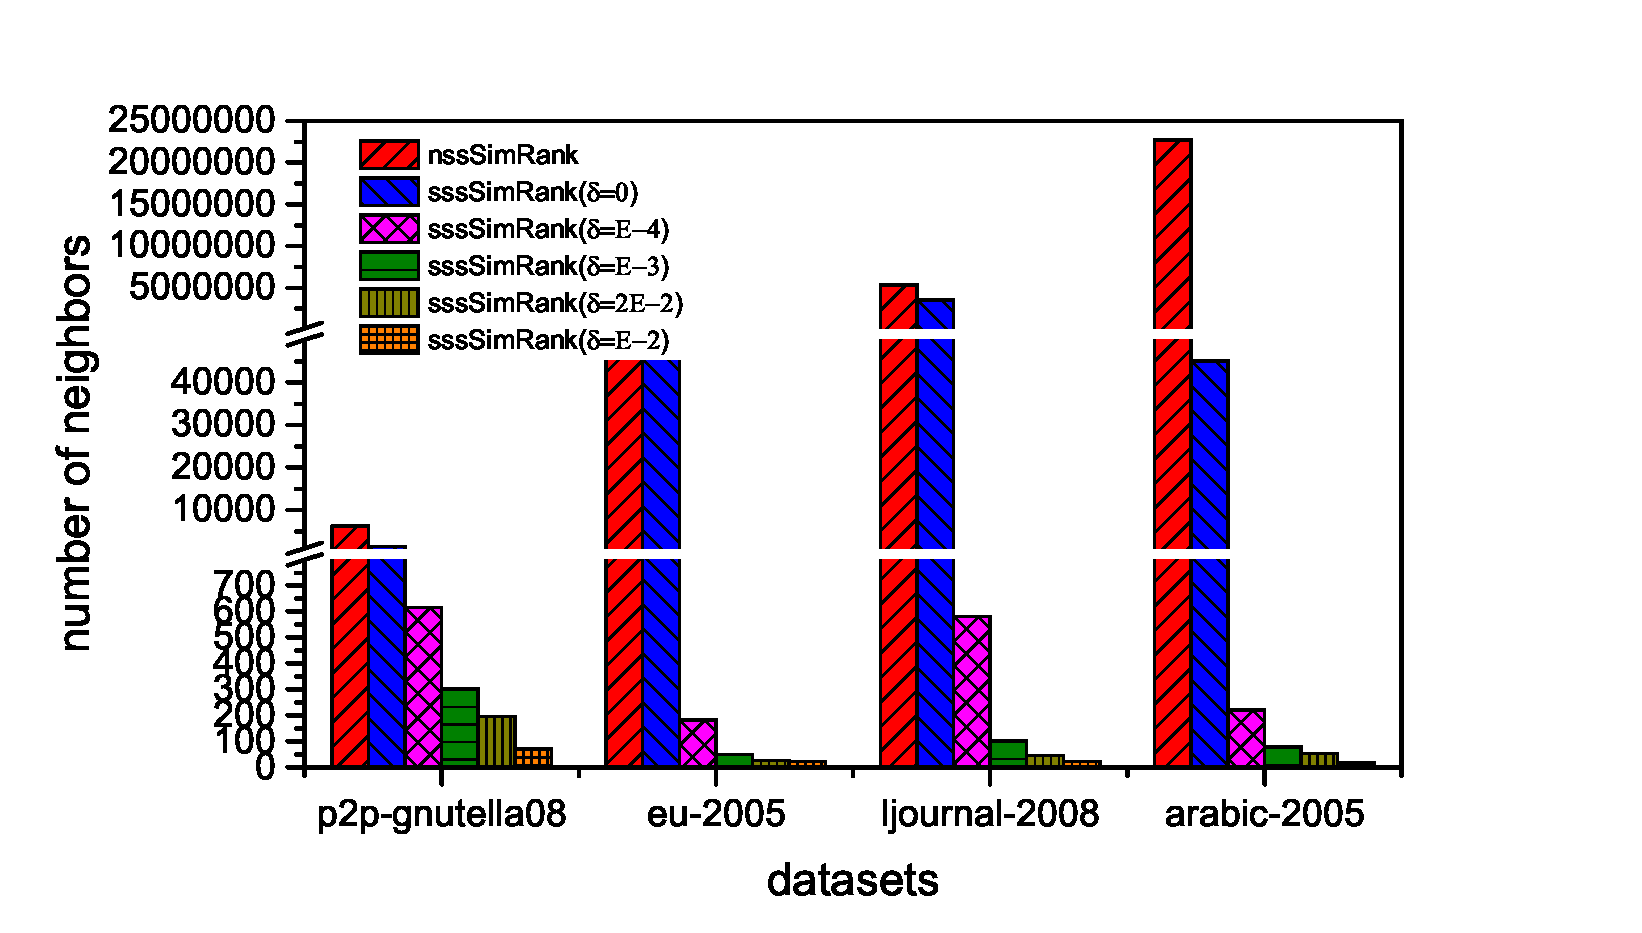
\includegraphics[width= 1\textwidth]{figure/neighborhoods.eps}\\
  \caption{生成领域数量的比较}\label{fig:ch1:runtime}
\end{figure}
从图中可以看出,sssSimRank极大地减少了生成领域的数量。
当$\delta=0$时,即算法没有筛除概率极小的游走时,领域数量减少了大约1500x倍。
从图中还可以观察到领域数量与概率阈值$delta$之间的关系。
当$\delta$越来越大时,意味这概率“筛子”的“孔”变得越来粗,幸存的随机游走会变得越来越少。
图\ref{fig:ch1:runtime}还表明,图eu-2005和arabic-2005减少领域的比例比图p2p-gnutella08和ljournal-2008要大很多,
这一观察同样表明算法中的概率筛子对稠密的图能更好地提高性能。
\subsection{算法的可扩展性}
我们考察分布式环境下算法的可扩展性。 首先考察算法运行时间随着输入图的大小的变化关系,结果如图\ref{fig:ch1:data_scalable}所示。
\begin{figure}[htbp]
  \centering
  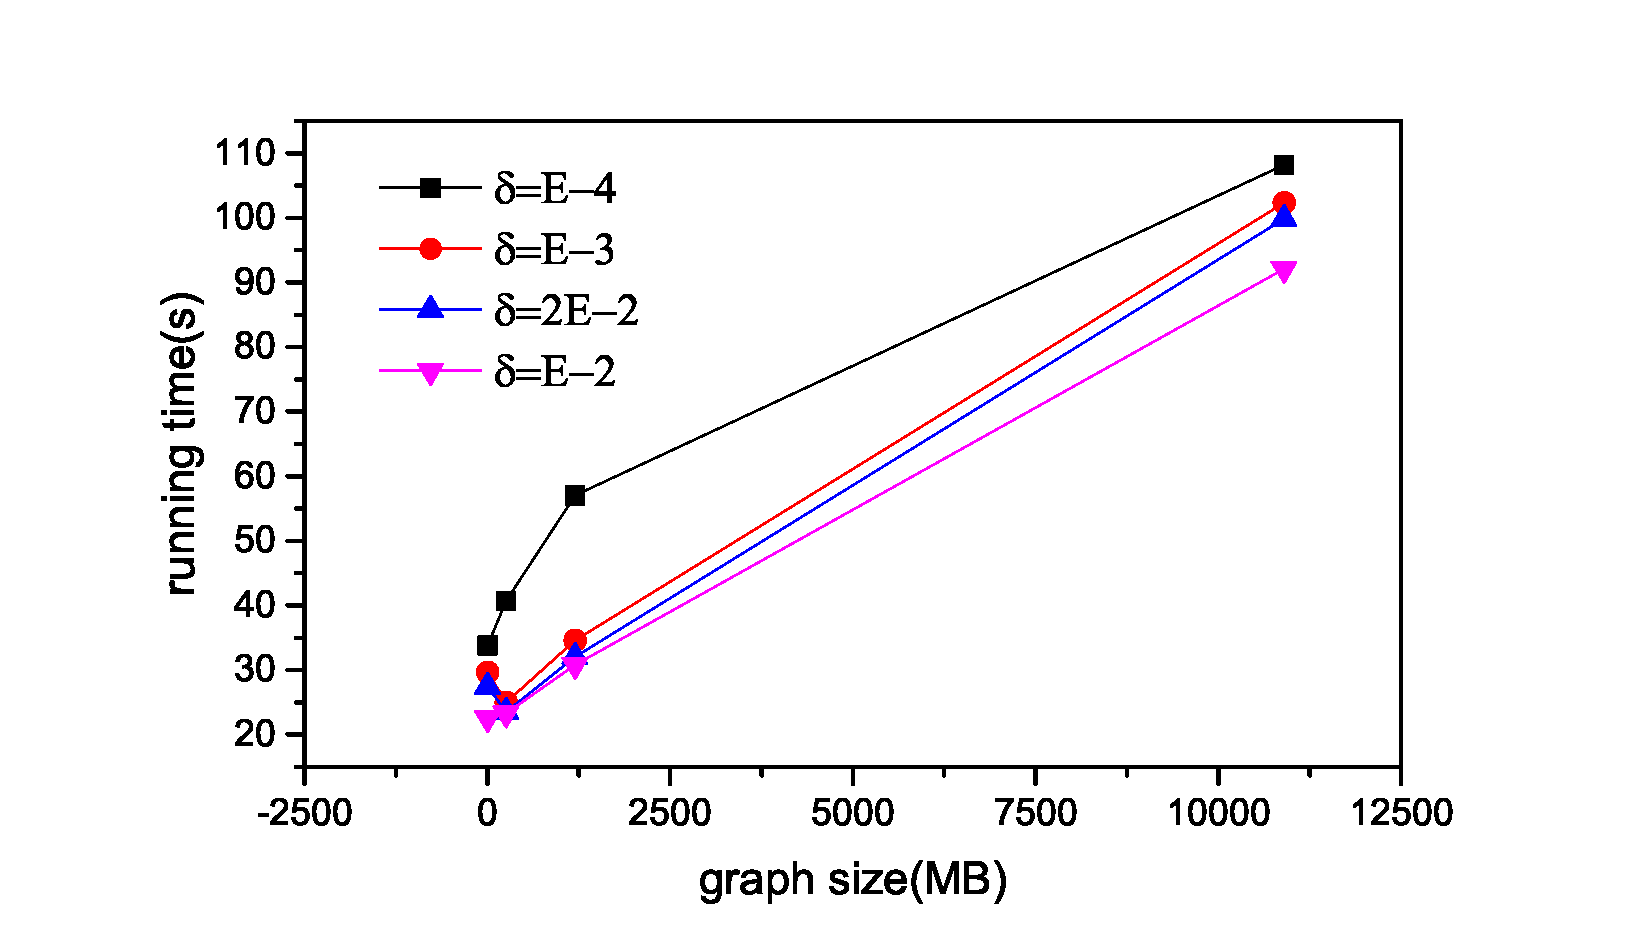
\includegraphics[width= 1\textwidth]{figure/data_scalability.eps}\\
  \caption{算法运行时间与输入图大小的变化关系}\label{fig:ch1:data_scalable}
\end{figure}

图中展示了当集群计算节点数目固定时,对于不同的$\delta$,运行时间随输入图规模大小变化的情况。 
可以看出,输入图的规模从215KB到10.9GB,而对应的运行时间基本上近似的随着输入规模大小线性的变化,
这一结论对不同的$\delta$都成立。这展示出sssSimRank良好的数据可扩展性。
我们还考察了当输入图的规模固定时,算法运行效率随集群中计算节点数量变化的情况。
所有的输入图使用同样的参数配置,$k=6$, $\delta=10^{-4}$。 计算节点数量从2增加到6。
注意到我们把$\delta$取得非常小,是因为$delta$越小,算法剔除的游走越少,算法的计算量越大。
这样更能提现计算量较为饱和的情况下算法的节点可扩展性。实验结果如图\ref{fig:ch1:node_scalable}所示。
从图中可以看到,对不同规模的输入图,算法的运行时间随集群计算节点的增加而近乎线性的减少,
这表面算法在分布式环境下具有良好的节点可扩展性。
\begin{figure}[htbp]
  \centering
  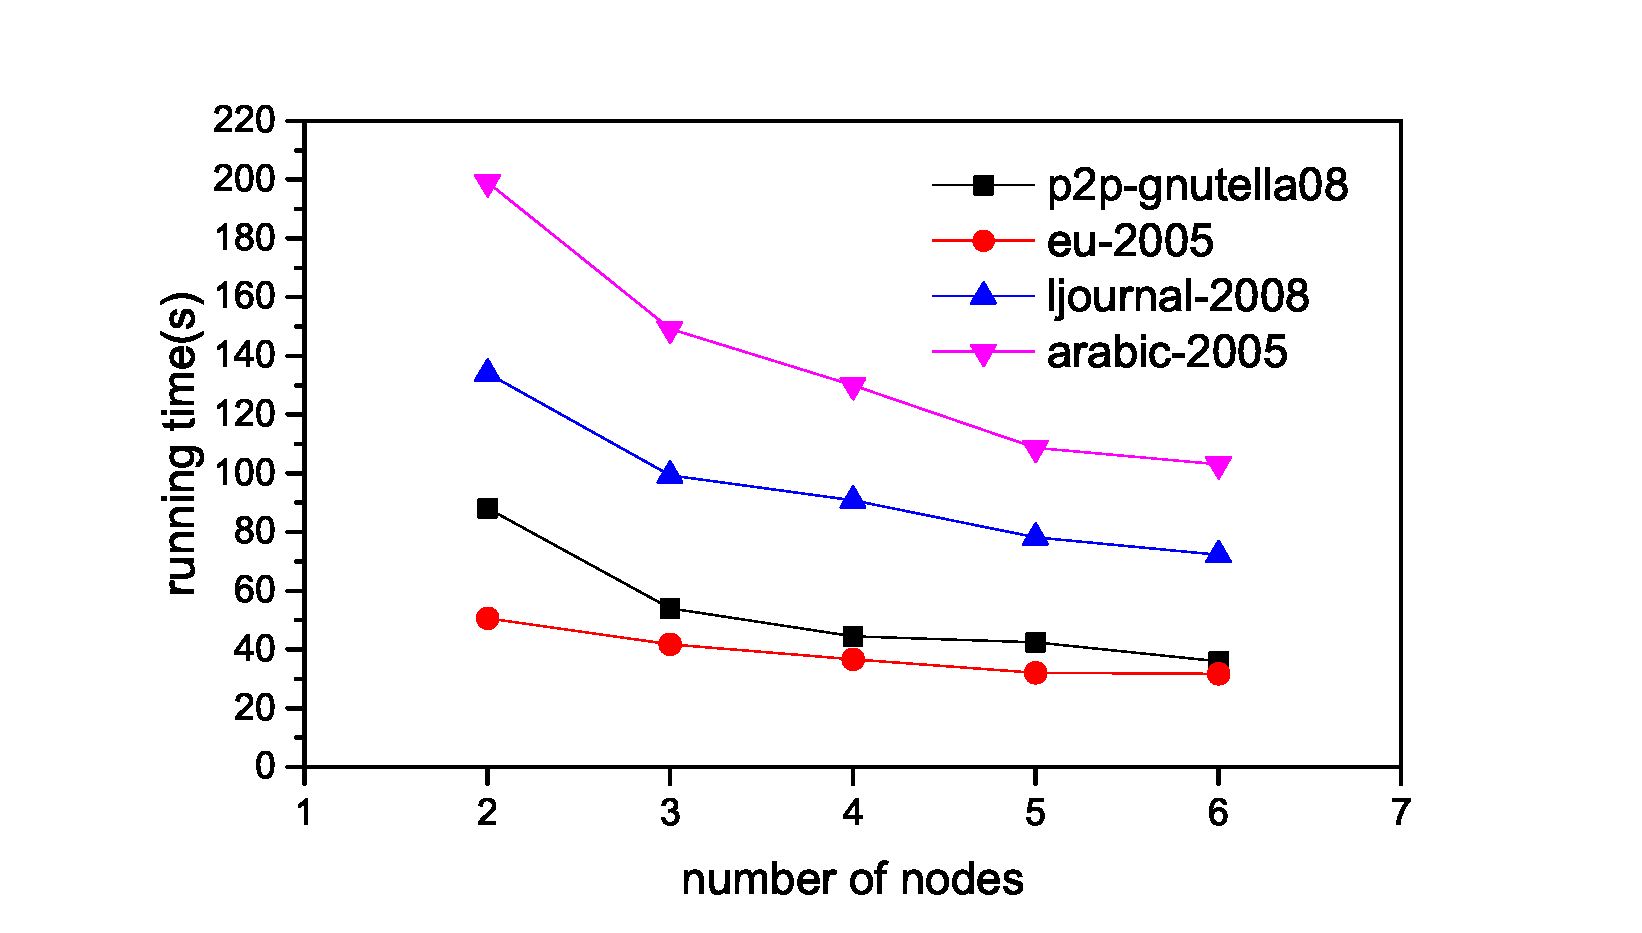
\includegraphics[width= 1\textwidth]{figure/node_scalability.eps}\\
  \caption{算法运行时间与集群计算节点数量的变化关系}\label{fig:ch1:node_scalable}
\end{figure}

\section{本章小结}
%%%%%%%%%%%%%%%%%%%%%%%%%%%%%%%%%%%%%%%%%%%%%%%%%%%%%%%%%%%%%%%%%%%%%%%%%%%%%%%
\chapter{分布式图分割方法}\label{chapter_graphpartition}
\section{概述}
随着现实生活中数据规模的不断扩大,与之对应的图数据网络结构愈加复杂,典型的大图甚至有数十亿个节点和上万亿条边。
普通的单台计算机由于运算内存的限制,远远无法承载大规模图数据的分析任务,
这给基于图计算的数据分析任务带来了巨大的挑战。
为了解决单计算节点计算问题有限的问题,最理性的方案就是利用分布式计算,
即将大规模图数据划分成多个子图装载到不同的分区或者不同计算节点上中,然后进行后续的图分析、图信息挖掘任务。

为了能够进行分布式图计算任务,必然会涉及到一个预处理步骤:将大规模图数据进行分布式划分。
图划分问题可以用数学语言描述如下:
\begin{definition}
 图划分(graph partitioning)。 给定一个图$G(V, E)$,设其顶点数量$|V|=n$,边的数量$|E|=m$,图的划分即将$V$划分为$k$个子集$(C_1, C_2, \dots, C_k)$,
使得对任意$1 \leq i,j \leq k$,有
\begin{equation}
\begin{aligned}
\label{eq:4-1}
 C_i \cap C_j=\emptyset \\
 \bigcup\limits_{i=1}^{k} C_{i} = V
 \end{aligned}
\end{equation}
给定一个划分,顶点在不同子集的边的权重(或数量)称作边割(edge-cut)。
\end{definition}
图划分问题往往还需要满足其他的约束条件,例如每个子集$C_i$的大小需要满足一定限制。
边割的大小揭示了划分是否最大程度地保留了原图中的稠密子结构,是衡量最终划分结果质量的重要标准,
因此通常图划分的目标函数里需要以某种形式最小化边割的大小。

作为图论领域的经典问题,目前已经有大量的工作对图划分做了各式各样的研究。 
文献【23】证明,图划分是一个NP完全问题,通常无法在有限的时间内找到图划分的最优解。
对于大规模图数据而言,将图中的顶点划分为不同的分块并将其存储到集群中不同的计算节点上去,
这一过程中每个计算节点为了能够访问到非本地存储的拓扑信息,必然会产生网络开销。
因此,采用什么样的方法对图分割,对划分过程中的网络开销、负载均衡、划分质量有着决定性影响。
大规模图数据的划分任务面临着许多新的挑战:
\begin{enumerate}
 \item 真实的图拓扑结构往往节点分布极不规则,这往往使得并行算法或分布式算法无法拥有很好的并发度或并行度
 \item 真实图的节点的度数往往表写出非常倾斜的分布,这使得不同处理器上的负载无法均衡
\end{enumerate}
因而设计一个好的分布式图划分方法具有重要的显示意义。
针对以上问题,我们提出一种高效的分布式图划分算法,实验结果表明,该方法具有较高的效率以及较好的可扩展性。

\section{相关工作}
目前学术界对图划分问题做了大量的一些研究,概括地说,目前的划分方法主要有以下几种:

\textbf{单节点串行算法。 } 文献【23】证明了图划分问题是一个NP完全问题。 
因此,早起很多工作都集中在设计一些近似算法以求得次优解。
文献【5】提出了Kernighan-Lin(KL)算法,该方法首先将图初始划分为偶数个分块,
然后基于一些启发式信息不断交换不同分块中的节点,直到不同划分之间的边割($edge-cut$)的权重之和达到最小。
KL算法每次迭代的时间复杂度为$O(n^3)$,它的划分质量较高,但是不能应用在超图上,而且对于规模稍大的输入图就显得无能为力。
FM算法【6】改进了KL算法中的顶点交换策略,每次不再交换一堆顶点而是改为基于分割线使得顶点在分割线两侧移动。
顶点移动的标准是最大化划分的负载均衡度。同时FM算法将算法的运用范围扩展到了超图(supergraph),它的每次迭代拥有线性的时间复杂度。
还有一些基于模拟退火【24】,遗传算法【25】的解决方案。
这些方法的研究对象都是基于内存存储的小图。

为了能够应对更大规模的图,一些多层次划分的方法相继被提出,包括 Metis[8],Chaco[7]和Scotch[10]。
这些方法主要由三个步骤组成:图的塌缩(coarsening phase)、初始划分(initial partition)、恢复(uncoarsening phase)。
其中,塌缩是指将图中若干顶点变为一个顶点,同时减少边的个数,从而提取出整个图拓扑信息的“骨骼”并基于此构造一个更小的图; 
初始划分指的是经过多次塌缩过程后,在小图上运行传统图划分算法得到一个原始划分;
最后恢复过程是按照塌缩步骤的相反顺序逐渐将图恢复成原来的形状,并将原始划分投影成原输入图上的划分。
这三个阶段缺一不可, 共同完成了从大规模图数据到简单小图再重新恢复的过程。
尽管可以处理的图规模有所扩大,它们的研究对象依然都是基于内存存储的小图。

\textbf{单节点并行算法。 } 为了进一步充分利用现代CPU的多核特性,从以上这些单线程算法中演化出一些并行化算法,
典型的有ParMetis[11],Pt-Scotch[12]等。 
这些算法或多或少地挖掘出图划分问题本身潜在的计算可并行性,所以其能够处理的图的规模也获得了的提升。 
但总的来说这些方法仍然是基于单计算节点的,其计算能力受到有限的计算资源的限制,对规模更大的(上百万节点)图无能为力。

\textbf{分布式图划分。 } 近年来,一些专门用于图计算的分布式平台越来越流行,包括Pregel[15],Giraph[X],Spark GraphX[TODO]等等。
这些平台的一个典型特点是支持以顶点为中心(vertex-centric)的编程范式,并且在系统层面拥有原生的顶点间消息通信机制。
然而上面几个流行的平台尽管也开放了一些接口支持用户按照需求设计自己的划分方法,但都没有提供一个直接可用的、高效的分布式图划分方法。
在读入输入数据时,它们往往使用随机划分的方法加载图数据,其划分质量没有任何保障。

\section{算法的基本框架}
我们从以下两方面来考虑图划分算法的优化目标:
\begin{enumerate}
 \item 划分结果的负载均衡。 考虑一个由$k$个计算节点组成的集群,因为存储资源(硬盘)散落在每个计算节点上,
 所以理想情况下最终划分的结果应当尽可能的均匀分布在集群中。也就是说,每个划分的大小应当在$\frac{|V|}{k}$左右,
 或者说划分过程中应该避免$|C| > \frac{|V|}{k}$的分块的产生。
 如果仍然有某个分块分布式地存储在超过一个结算节点上,那所谓的分布式图划分就没有意义。
 \item 划分结果的质量。 理想情况下图划分算法应该可以把图中稠密的子图归类于一个分块中。
 但是因为有负载均衡的限制,而图中稠密子图的规模天然是不均匀的,因此我们从整体考虑划分的质量。
 设$P$是图$G(V,E)$的一个划分,定义其边割为
 $W_{P}=\sum\nolimits_{e(u,v) \in E, u \in C_i, v \in C_j} w\big(e(u,v)\big)$,即所有连接不同分块的边的权重之和。
 理论上,$W_P$应尽可能的小。
\end{enumerate}
我们的算法借鉴多层次划分的思想,即通过不断的coarsen步骤使得原图的规模越来越小,
当图的规模小到某个可以接受的阈值时,再使用KL或FM等单节点算法直接进行划分。
最后划分的结果再直接投影到原图中,这样就得到了最终的划分结果。
图\ref{fig:mlp_framework}揭示了多层次划分算法的大致框架。
\begin{figure}[htbp]
  \centering
  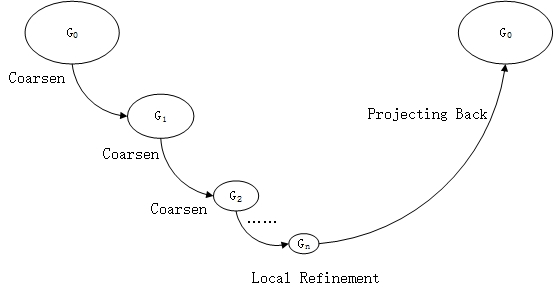
\includegraphics[width= 0.75\textwidth]{figure/coarsen.jpg}\\
  \caption{多层次图划分的算法框架}
   \label{fig:mlp_framework}
\end{figure}

\subsection{塌缩步骤}
设原始输入图为$G_{0}(E_0,V_0)$,并假设迭代塌缩过程中产生的中间图由记号$G_1, G_2, \dots, G_t$表示。
相应的,由中间图产生的划分称作$P_1, P_2, \dots, P_{t}$。
注意到迭代过程中图的划分与其输入图下标是对应的,即$G_{i-1} \rightarrow P_i \rightarrow G_i$。
我们首先给出塌缩的具体过程。
\begin{definition}
塌缩图的拓扑结构。 迭代塌缩过程中,给定图$G_i(V_i, E_i)$上的划分$P_i=(C_1, C_2, \dots, C_n)$,基于$P_i$上构造塌缩图$G_{i+1}(V_{i+1}, E_{i+1})$如下:
 令$V_{i+1} = P_i$,即$P_i$中的每一个划分对应$G_{i+1}$中的一个新顶点;边$(C_i, C_j) \in E_{i+1}$当且仅当$\exists
 u \in C_i, v \in C_j$ 并且 $(u, v) \in E_i$。
\end{definition}
通过这样的塌缩过程,显然有$|V_{i+1}| < |V_i|$,也就是说图的规模在迭代中不断变小。
经过反复塌缩后,图$G_i$的规模会降低到某个阈值以下。
\begin{definition}
塌缩图的权重。 设初始输入图$G_{0}(V_0,E_0)$中每个顶点有单位权重$w_u=1$,每条边$(u,v)$同样有单位权重$w_{u,v}=1$。
设迭代过程中基于图$G_i$构造塌缩图$G_{i+1}$,并且有$V_{i+1}=(C_1, C_2, \dots, C_n)$,
那么新的图中顶点$u$的权重定义为:
\begin{equation}
\label{eq:vertex_weight}
w(u) = \sum\limits_{v \in C_k} w(v)
\end{equation}
其中,$C_k$为图$G_{i+1}$中新顶点$u$在图$G_i$中对应的分块。
类似的,边$e=(C_i, C_j)$的新权重定义为:
 \begin{equation}
w(C_i, C_j) = \sum\limits_{e(u,v) \in E_i, u \in C_i, v \in C_j} w\big(e(u,v)\big)
\end{equation}
即压缩图中的新边的权重等于该边在原图中代表的两个分块间所有相连接的边的权重之和,而新顶点的权重为原图中对应分块中的所有顶点的权重之和。
\end{definition}
通过这样的权重赋值方式,保证了塌缩后的图具有如下特性:
\begin{enumerate}
 \item 边的权重赋值方式使得划分塌缩后的图所的边割代价与划分原图保持一致,这样可以保证图划分质量的一致性。
 \item 顶点的权重赋值方式使得划分塌缩后的图的负载均衡状况与划分原图保持一致,这样可以保证划分过程中负载均衡的一致性。
\end{enumerate}

那么,迭代过程中如何基于$G_{i-1}$生成划分$P_i$呢?
ParMetis【】基于最大匹配(maximal match)来对图进行压缩。匹配指的是图中边集$E$的子集,其中每条边的端点两两不相交。
如果一个匹配无法再加入其他边,那么这个匹配就是一个最大匹配。
具体进行塌缩时,ParMetis采取的做法是对匹配中的边,直接将其两个端点融合成一个新的顶点;而不在匹配中的顶点继续保留,这样就可以产生塌缩后的图。
选择最大匹配的目的是最大程度地通过塌缩减小图的规模。

文献【todo】给出了一种基于标签传播(Label Propogation,LP)的图划分思路。
LP算法被广泛运用于解决社区发现(Community Detection)问题。
社区,从直观上来看指的是网络中的一些密集群体,每个社区内部的顶点间的联系相对紧密,但是各个社区之间的连接相对来说却比较稀疏。
社区发现任务与图划分任务的区别在于,前者不会固定社区的数量,因为具体社区的个数是由输入图的内在结构决定的;
而后者往往会设定需要划分的分块个数$k$。
两者的相似之处在于,社区检测过程中图中局部联系紧密的子结构往往会共享同一个社区ID,这与图划分任务的内在要求相一致。
与其他图塌缩方法(例如最大匹配)相比,基于社区检测的方法能够更好地感知原图中的语义。

LP算法的思想非常简单:最初的时候我们给图中每个顶点一个单独的社区ID,
然后我们迭代式地为每个顶点更新社区ID。
每次迭代中,每个顶点将其邻居顶点所属社区ID出现次数最多的那个作为自己新的ID。
当$G$中每个顶点的社区ID基本上不再变动时,算法结束。
图\ref{fig:mlp_cd}展示了一个典型的社区发现结果。
从图中可以直观的看到算法总共检测到了4个社区。如果直接将其当做图的一个4划分$P=(C_1, C_2, C_3, C_4)$,其划分质量也是不错的。
\begin{figure}[htbp]
  \centering
  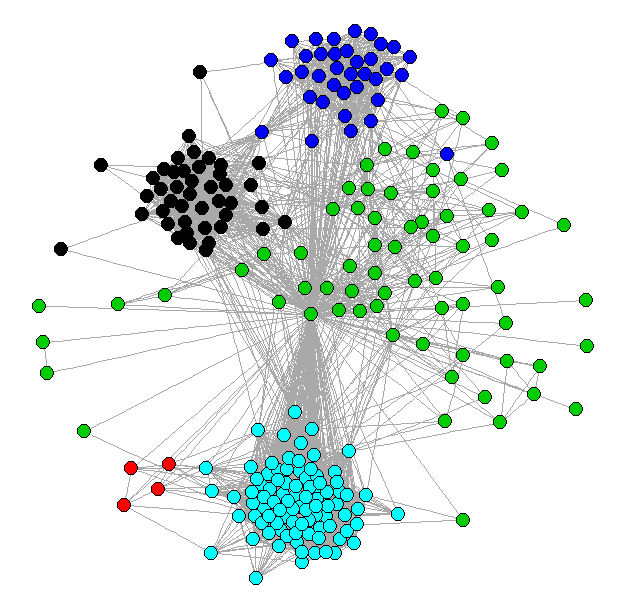
\includegraphics[width= 0.6\textwidth]{figure/lp.png}\\
  \caption{社区发现算法的结果,不同颜色代表不同的社区ID}
   \label{fig:mlp_cd}
\end{figure}

上述社区发现过程中,确定每个顶点所属的社区ID并没有使用$G$中任何的先验信息或者是既定的目标函数,
而只是利用了图中顶点与其邻居顶点的局部相似性原理。
而确定每个顶点所属社区ID这一步骤是迭代过程中的计算主体,因此有很搞的提升空间。

本文借鉴了文献【7】中模块度(modularity)的思想,试图在迭代过程中有方向性地寻找合适的社区ID。
模块度是常用的一种衡量网络中社区稳定度的方法。
简而言之,对于一个已经分配好社区(或划分)的图,分配在同一社区的边占总边数的比例,与对这些边随机分配得到的概率期望,这两者的差就是其模块度。
用数学预言描述,设$d_v$表示顶点$v$的度数, $C_v$表示节点$v$所在社区的ID,图的模块度的定义如下:
\begin{equation}
\label{eq:mod}
Q = \frac{1}{2W}\sum\limits_{u, v \in V} \left[w_{u,v} - \frac{{d_u}{d_v}}{2W} \right]\delta \left(C_u, C_v\right),
\end{equation}
其中$\delta(C_u, C_v)$表示顶点$u, v$是否处于一个社区,即如果$C_v = C_u$,那么$\delta(c_u, c_v)$等于1;否则为0。
$w_{u,v}$表示边$(u,v)$是否存在,即如果$(u,v)\in E$,那么$w_{u,v}=1$,
否则为0。$W$表示图中所有边的权重之和,即$W=\sum_{(u,v) \in E}w_{uv}$。

按照上面的定义,我们有如下的定理:
\theorem{根据上面的定义,我们实际上可以得到模块度$Q$定义的简单形式:
\begin{equation}
Q = \sum\limits_{c \in P} \left[\frac{I_c}{2W} - {\left(\frac{S_c}{2W}\right)}^2 \right]
\end{equation}
}
其中,$I_c$表示ID为$c$的社区中两个端点都在$c$中的边的权重之和,而$S_c$表示社区$c$中所有顶点的度数之和,
即$S_c = \sum_{v \in V} {d_v}$
\begin{proof}
根据\label{eq:modularity}的定义,如果顶点$u, v$属于不同社区的话,那么显然有$\delta(C_u, C_v)=0$,
因此只要考虑属于同一社区的点对,即我们可以把公式\ref{eq:mod}改写为:
\begin{equation}
\begin{aligned}
Q &= \frac{1}{2W}\sum\limits_{u, v \in V} \left[w_{uv} - \frac{{d_u}{d_v}}{2W} \right]\delta(C_u, C_v) \\
& = \frac{1}{2W}\sum\limits_{c \in P} {\sum\limits_{u, v \in c} { \left[w_{uv} - \frac{{d_u}{d_v}}{2W} \right]}} \\
& = \frac{1}{2W}\sum\limits_{c \in P} \left[{\sum\limits_{u, v \in c} { w_{uv} - \frac{\sum\nolimits_{u,v \in c}{{d_u}{d_v}}}{2W}}}\right] 
\end{aligned}
\end{equation}
注意到有$I_c=\sum\nolimits_{u, v \in c}  w_{uv}$, 
并且有$\sum\nolimits_{u,v \in c}{{d_u}{d_v}} =
\sum\nolimits_{u \in c}{d_u} \sum\nolimits_{v \in c}{d_v} = S_c S_c = {S^2_c}$。
因此,我们有如下的定理:
\begin{equation}
\begin{aligned}
Q &= \frac{1}{2m}\sum\limits_{c \in C} \left[I_c - \frac{S_c^2}{2m} \right] \\
& = \sum\limits_{c \in P} \left[\frac{I_c}{2m} - {\left(\frac{S_c}{2m}\right)}^2 \right]
\end{aligned}
\end{equation}
\end{proof}


\begin{figure}[t]
    \centering
    %\subfig[fjalkf]
    \begin{subfigure}[b]{0.48\linewidth}        %% or \columnwidth
        \centering
        \label{fig:two:one}
	\resizebox{!}{!}{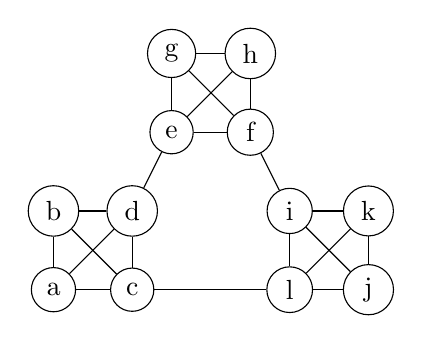
\begin{tikzpicture}
\tikzset{vertex/.style = {shape=circle,draw,minimum size=10 pt}}
\tikzset{edge/.style = {-,> = latex'}}
% vertices
\node[vertex] (a) at  (0,0) {a};
\node[vertex] (b) at  (0,1) {b};
\node[vertex] (c) at  (1,0) {c};
\node[vertex] (d) at  (1,1) {d};

\node[vertex] (i) at  (3,1) {i};
\node[vertex] (j) at  (4,0) {j};
\node[vertex] (k) at  (4,1) {k};
\node[vertex] (l) at  (3,0) {l};

\node[vertex] (e) at  (1.5,2) {e};
\node[vertex] (f) at  (2.5,2) {f};
\node[vertex] (g) at  (1.5,3) {g};
\node[vertex] (h) at  (2.5,3) {h};
%edges
\draw[edge] (b) to (a);
\draw[edge] (b) to (c);
\draw[edge] (a) to (d);
\draw[edge] (b) to (d);
\draw[edge] (c) to (a);
\draw[edge] (c) to (d);

\draw[edge] (e) to (h);
\draw[edge] (e) to (f);
\draw[edge] (e) to (g);
\draw[edge] (f) to (h);
\draw[edge] (f) to (g);
\draw[edge] (g) to (h);

\draw[edge] (i) to (l);
\draw[edge] (i) to (k);
\draw[edge] (i) to (j);
\draw[edge] (l) to (k);
\draw[edge] (l) to (j);
\draw[edge] (j) to (k);


\draw[edge] (f) to (i);
\draw[edge] (d) to (e);
\draw[edge] (c) to (l);
\end{tikzpicture}
}
	\caption{$G$}
	\label{fig:figure2:figure1} 
	\end{subfigure}
    \begin{subfigure}[b]{0.48\linewidth}        %% or \columnwidth
     \centering
	\resizebox{!}{!}{\input{temp6.tikz}}
	\caption{经过塌缩后的图$G\prime$}
	\label{fig:figure2:figure2}
    \end{subfigure}
    \caption{(a)为一个简单的示例图,(b)为改图经过塌缩(coarsen)后的图$G\prime$, 每个顶点代表$G$中的一个划分}
    \label{fig:two}
\end{figure}
我们下面给出基于模块度优化的图划分方法。
迭代初始化时每个顶点拥有一个单独的ID,考虑把某个顶点$u$重新放入到某个新的分块$C$后,整个图$G$的模量会发生变化,
我们用符号$\Delta Q_{u,C}$表示。
根据模量的定义,我们有:
\begin{equation}
\begin{aligned}
 \Delta Q_{u,C}=\left[ \frac{I_c+w_{u,C}}{2W} - {\left(\frac{S_C + d_u}{2W} \right)}^2 \right] -
 \left[ \frac{I_C}{2W} - {\left(\frac{S_C}{2W} \right)}^2 \right] - {\left(\frac{d_u}{2W}\right)}^2 
\end{aligned}
\end{equation}
其中,$w_{u,C}$指的是顶点$u$指向分块$C$中的所有的边的权重之和。经过若干步骤的化简,最终我们可以得到模块度变化的简单形式:
\begin{equation}
\begin{aligned}
\label{eq:deltaQ}
 \Delta Q_{u,C}=\frac{w_{u,C}}{2W} - \frac{S_Cd_u}{2W^2} 
\end{aligned}
\end{equation}
上式告诉我们,将某个顶点从之前的分块移除并重新放入新的分块之中时,只需考虑图中的局部信息就可以计算出模块度的变化量,
而不需要按照式\ref{eq:mod}那样暴力遍历所有边。

因为Spark平台内部RDD的计算无法按照异步(asynchronize)方式生成,
即在第$t$轮迭代中计算维护图中顶点的相关信息只能基于第$t-1$轮迭代各顶点已有的信息,
每次迭代时所有的顶点一并计算更新。
Spark需要严格同步(synchronize)本轮迭代中所有线程的计算结果,才会进入下一步的迭代。
基于这个特性,我们对图进行基于模块度优化的塌缩算法如\ref{alg:mlgp}所示。
算法包含三个参数,$\alpha, \beta, k$。
其中,$\alpha$指的是反复塌缩过程的目标划分数目,如果迭代过程中当前的划分数目大于$\alpha$,就继续迭代下去。
$\alpha$的取值与第二步中单节点图划分算法可以处理的输入图规模有关。
$\beta$指的是我们基于模量的塌缩方法的迭代次数。
参数$k$控制了图划分过程中每个分块大小的上限$|V|/k$。
如果$k$设置得较大,那么最终每个分块规模会比较小,而分块数目较多;
如果$k$设置得较小,那么每个分块规模可能较大,而分块数目较少。
首先根据参数$k$求出分块大小的阈值$bs$(第2行),并且初始时赋予图中每个顶点一个不同的ID(第3行)。
算法会一直迭代直到当前的分块数目小于$\alpha$(第4行),每次迭代过程中都会更新划分$P$并生成新的塌缩图(第18-19行)。
每次的迭代内部包含一个迭代$\beta$次的社区发现过程(第6-17行)。
如果模块度有增益,那么一个顶点会移入到其邻居顶点所属的社区中(第8-17行)。
注意到如果待加入的那个社区中包含的顶点权重之和(根据公式\ref{eq:vertex_weight},权重之和表示该社区在原输入图$G_0$对应的顶点数目)
已经超出了分块阈值$bs$,那么该社区不会接受新的顶点加入(第10行)。
这保证了最终分块的负载均衡,即每一个分块的顶点数目都不会超过$bs$。

%\begin{figure}[tbp]
\begin{algorithm}[h]
\captionof{algorithm}{Modularity-based Graph Coarsening}
\label{alg:mlgp}
\begin{algorithmic}[1]
\Procedure{GraphCoarsening}{$G, \alpha, \beta, k$}
  \State {Set block size threshold $bs \gets |V|/k$};
  \State Initialize partition $P$, which assigns each vertex a unique partition ID;
      \While{$|V| \ge \alpha$} \Comment{\#Paritions greater than  $\alpha$}
	  \State $W \gets \sum\nolimits_{u,v \in V} w_{u,v}$; 
	  \For{$i=1$ to $\beta$}
	    \For { $u \in V$}
		\State{$maxGain \gets -1$};
		\For{ $v \in N_v$}
		  \If {$|C_v| \ge bs$} \Comment{Partitions with size smaller than $bs$}
		     \State $\Delta Q_{u,C_{v}} \gets \frac{w_{u,C_v}}{2W} - \frac{S_{C_v}d_u}{2W^2}$;
		     \If {$\Delta Q_{u,C_{v}} > maxGain$}
		      \State $maxGain \gets \Delta Q_{u,C_{v}}$
		      \State $newPartition \gets v$
		     \EndIf
		   \EndIf
		\EndFor
		\If {$maxGain > 0$}
		    \State $C_{newPartition} \gets C_{newPartition}\cup\{u\}$;
		    \State $C_{u} \gets C_{u} - \{u\}$;
		    
		\EndIf	
	    \EndFor
	  \EndFor
	  \State update $P$
	  \State {$G \gets $ the coarse-grained graph constructed from $P$}
	\EndWhile
\State \textbf{return} $G$.
\EndProcedure
\end{algorithmic}
\end{algorithm}
%\end{figure}

\subsection{初始划分与恢复步骤}
经过反复塌缩后,原图$G_0(V_0,E_0)$变成了规模足够小的图$G_t(V_t,E_t)$,其中$|V_t| < \alpha$。
此时$G_t$中每个顶点$u$都对应原图$G_0$中的若干紧密连接的顶点集合$C_u$,$u$的权重对应$|C_u|$;
$G_t$中的每条边$(u,v)$都对应$G_0$中顶点集合$C_u$与$C_v$之间的边割,$(u,v)$的权重对应边割集中边的数目。
因此,对$G_t$的划分$P_t$可以一一对应到对$G_0$的划分$P^\star$。
并且,顶点$u \in V_t$是$P_t$的最小划分单元,而对应到$G_0$中,集合$C_u$才是$P^\star$的最小划分单位。
$C_u$中的顶点是不可重新进行划分的,因为它们的分块在之前的塌缩过程中就已经由基于模块度的社区发现逻辑决定了。

我们直接使用METIS软件包提供的单节点算法求解$G_t$的划分$P_t$。
具体求解时,仍然按照之前的目标:即划分的负载均衡以及边割权重的最小化。
因为METIS只能处理规模较小的图,所以$\alpha$的值应当设置在合理的范围内。

恢复过程比较简单,对$P_t$中的每个顶点$u$,直接把其在$G_0$中一一对应的顶点集合$C_u$中的所有顶点的分块号,
设置为$u$在$P_t$中的分块号即可。


\begin{algorithm}[H]
\captionof{algorithm}{Multi-Level Graph Partitioning}
\label{alg:mlgp}
\begin{algorithmic}[1]
\Procedure{MultiLevelGraphPartition}{$G, \alpha, \beta, k$}
	\While{\#partitions $\ge \alpha$}
		\State $P \gets $ results of modularity-based community detection for $\beta$ iterations;
		\State Construct $G\prime$ from $P$; \Comment{Coarsen.}
	\EndWhile  
	\State $P_1 \gets $ Run local graph partitioning on $G\prime$. \Comment{Final refinement.}
	\State restore partition $P\prime$ from $P_1$ \Comment{Project back to the orignal graph.}
\EndProcedure
\end{algorithmic}
\end{algorithm}

\section{基于Spark平台的算法的实现}
我们主要基于Spark提供的分布式图计算框架GraphX来实现算法的逻辑。
因为图中顶点在计算过程中需要与相邻顶点通过网络交换信息,我们首先给出顶点的定义:
\begin{figure}[h]
\begin{lstlisting}[caption={My Caption},captionpos=b]
class Node extends Serializable{
    val vID:Long
    val pID:Long
    var weight:Double = 1.0,
    var pWeightSum:Double = 0.0,
    var nbrPWeightSum:Double = 0.0
    var modularity:Double
    ...
}
\end{lstlisting}
  \caption{简化的Node结构体}
\end{figure}
可以看到,Node这个结构记录了顶点的ID、所属分块ID、权重、顶点到所属分区的连接数、顶点到邻居分区的连接数等信息。
这些信息在计算过程中会不断的在顶点之间传输、交换、维护。

GraphX具体的编程范式比较复杂,但是总的来说,算法工作的流程是在Map阶段所有顶点向其邻居顶点发送自己包含本身信息的消息,
这些消息经过本身包含(srcID, dstID),发送至同一目的顶点的若干消息经过Spark内部的Partitioner之后组装成消息列表准确发送至目的地。
目标顶点收到这些消息后,在本地进行必要的计算就获得了周围顶点的必要信息,然后就可以根据公式\ref{eq:deltaQ}计算出$\Delta Q$的大小。
\begin{figure}[h]
\begin{lstlisting}
var graph = Graph(vertexRDD, edgeRDD)
while(run) {
    var newVertexRDD = graph.aggregateMessages()
    var tmpGraph = Graph(newVertexRDD, graph.edges)
    var edges = generateEdges(tmpGraph)
    graph = Graph(newVertexRDD, edges)
    num = graph.vertices.filter().count()
    run = if {num == 0} True else False
    ...
}
\end{lstlisting}
  \caption{程序运行逻辑}
\end{figure}
其中,$generateEdges$是塌缩过后重新生成规模更小的图的过程,其具体细节如下所示:
\begin{figure}[h]
\begin{lstlisting}
graph.triplets.map{
  t => Edge(t.srcAttr.pID, t.dstAttr.pID, t.attr)
	.flatMap {
	    e => {
	      ...
	      List()
	    }
	}.reduceByKey()
	 .map{
	    e => Edge(new Node(), new Node()) //construct new edge
	    }
}
\end{lstlisting}
\caption{塌缩过程中生成新的边}
\end{figure}
我们首先统计有哪些边在当前图中横跨了不同的分块,然后使用reduceByKey操作把这些边变成变成一条新的边,
这个过程中变得数量大大地减少了,并且新边的权重,以及新边两边端点的权重,都同时被更新了。
\section{实验评估}
\section{本章小结}
%%%%%%%%%%%%%%%%%%%%%%%%%%%%%%%%%%%%%%%%%%%%%%%%%%%%%%%%%%%%%%%%%%%%%%%%%%%%%%%
\chapter{分布式全点对相似度计算方法}\label{chapter_allSimRank}
\section{概述}
上一章节描述了计算单源点SimRank相似度的计算方法,如果进一步地考虑计算图$G$中全点对的相似度,
那么不管是直接根据SimRank的定义采用矩阵迭代计算的方法,还是将全点对计算问题简单看做$|V|$个单源点相似度计算问题,
整个计算的开销无疑是不可承受的。
考虑一个现实生活中的拥有数百万节点的大规模图,其邻接矩阵的元素规模达到万亿级别($|V|^2$),
涉及到这么大规模的矩阵乘法需要做复杂的算法设计和程序优化,甚至需要有专门的高性能超算平台来配合程序的运行。
如果简单地将全点对相似度计算看做$|V|$个单源点计算问题,那显然没能够充分挖掘出问题内在的可并行性。
因此,需要重新设计设计高效的算法来计算图$G$中全点对的相似度。
本文总体的算法思路是“分而治之”的思想,
试图将复杂的计算任务分解为如果如果更小、更容易处理的子任务。
而本章将重点叙述其中的“分解”步骤:图划分,作为一个重要的中间步骤,分割的质量、效率直接关系到最终全点对相似度的计算效果。
\section{相关工作}
为了方便叙述, 我们用$n$表示输入图的节点个数,用$m$表示图的边的个数,用$d$表示图中节点的平均度数。 
对于迭代算法,使用$k$表示算法需要迭代的次数。

\textbf{基于矩阵乘法的计算方法}。 Jeh和Widom提出了第一个基于矩阵乘法的SimRank迭代计算方法,改算法计算全点对的相似性,其复杂度为$O(kn^2d^2)$
.[9]随后通过剪纸、局部访问等技术在矩阵乘法层面将算法的时间复杂度提升到$O(kn^2d)$。【10】使用了快速矩阵乘法来加速计算过程。
文献【12】进一步将算法的时间复杂度提高到$O(kn^2d^{\prime})$,其中$d^\prime < d$。
文献【13】提出了一种基于Keonecker乘积和矩阵奇异值分解(SVD)的非迭代算法,该算法首先在$O(r^4N^2)$时间内计算一些出辅助矩阵,其中$r$是
输入图的领接矩阵的秩,然后再在$O(r^4N^2)$时间内获取给定源点与其他所有节点的相似性。
文献【14】使用了GPU来加速矩阵的计算速度。
对于单点对的SimRank计算,文献【11】给出了一个时间复杂度为$O(kd^2\cdot \min{\{n^2, d^k\}}$的算法。
文献【15】进一步地通过使用概率方法将时间复杂度提高到$O(km^2-m)$。

\textbf{基于随机游走的计算方法}。
图中节点$v$,$u$的相似性,可以解释为:以节点$u$和节点$v$分别为初始点,同步移动的随机游走第一次在某个节点相遇的概率的期望值。
文献【16】给出了第一个基于随机游走的算法, 该算法首先建立一个大小为$O(nN)$的$N$个随机游走的“指纹”索引,然后基于索引查询单点对的相似性。
文献【17】提出一种在随机游走中使用采样技巧计算单点对相似性,该方法在允许一定精度损失的情况下提高了计算效率。
文献【18】研究了图中top-$k$个最相似点对的查询问题,其中$k$往往是一个非常小的值。
该方法把单点对相似查询问题转变为规模为$G\times G$的乘积图上的查询问题。

\textbf{分布式计算方法}。 文献【19】提出了一种基于增量变化的$Delta-SimRank$算法。该算法发现,SimRank可以改写为一种迭代的增量计算方式,
即迭代过程中,不直接改变点对之间的相似性而是计算相对于上一轮迭代的增量。该方法充分利用了迭代计算过程中很多点对间相似性增量为0的事实,减小了
计算过程中的数据传输量。
文献【20】提出了一种基于Spark平台的分布式计算方法,该方法打破了计算点对相似性之间的递归依赖关系:首先线下计算一个不变矩阵$D$,然后线上根据$D$使用
蒙特卡洛方法快速给出查询。然而,$D$的计算被当做一个解线性方程组的过程,这在分布式环境下非常低效,因此虽然算法线上查询的效率很高,
但线下预处理的时间开销非常巨大。
\section{算法框架}
基于章节\ref{chapter_graphpartition}中对图做出的划分,我们现在给出一个计算全点对相似度的近似算法。
文献【11】描述了一种基于图中分块结构(Block Structure)的若干性质来加速计算PageRank的方法,我们的近似算法直接受到了该算法的启发。
对于现实生活中的图数据集,图中天然可以划分为着若干稠密的分块,这些稠密的分块包含了更多节点之间的连接,
因此往往也蕴含着最多的人们感兴趣的信息。本文正是充分利用了这一性质,提出了一种计算全点对相似度计算的近似算法。
相比原来的SimRank的计算方法,该算法不仅极大地提高了计算效率,而且保留了原来的计算精度。

在计算节点对之间的相似性时,节点对可以分为两种:
\begin{enumerate}
 \item 位于同一稠密分块之中的顶点对。 在上一章节中,我们已经详细介绍了将原图$G$划分为若干稠密分块的方法,每一个划分好的
 分块都被存放在集群中的某一个计算节点中。 这种情况下可以\ref{eq:two}中的串行计算方法直接计算出该点对的相似性。
 \item 位于不同分块之中的顶点对。这种情况下,注意到因为两个顶点分别处于不同的稠密分块之中,这意味这两个顶点的距离会以较大概率地比较远,
 也即意味着这两个顶点的相似性会较大概率地在数值上表现得非常之小。这个时候我们通过估算近似地给出最终的相似度。
\end{enumerate}
与上一章节类似,假设图中的每一个分块是一个顶点,那么图的划分就形成了一个塌缩图。
基于这个塌缩图,我们首先定义图中边的权重:
\begin{definition}
 塌缩图中边的权重。 假设对图$G$有划分$P=(C_1, C_2, \dots, C_n)$,
 设$L(C_i)$表示分块$C_i$中所有边的数量,包括该分块内部的边以及连接到其他分块的边;
 $L(C_i, C_j)$表示分块$P_i$与分块$P_j$中相连接的边的数量。
 设图$G^\prime$为划分$P$形成的塌缩图,$v_i \in G^\prime, v_j \in G^\prime$, 
 且$v_i$为分块$C_i$对应的顶点,$v_j$为分块$C_j$对应的顶点。
 那么定义边$(v_i, v_j)$的权重为:
\begin{equation}
 w(v_i, v_j) = \frac{L(C_i, C_j)}{L(C_i)} 
\end{equation}
$v_i$自己到自己的权重定义为
\begin{equation}
 w(v_i, v_i) = 1-\sum_{v_j \in O(v_i)}{w(v_i, v_j)}
 \end{equation}
显然,一般情况下$w(v_i, v_j)$与$w(v_j, v_i)$是不同的。
\end{definition}
这样经过塌缩后的图$G^\prime$变成了一个加权有向图。
边$(v_i, v_j)$的权重可以粗略理解为某个随机游走者从点$v_i$“逃逸”到点$v_j$的概率。
$w(v_i, v_j)$越大,说明在原图$G$中分块$C_i$与$C_j$的交叉边越多,联系越紧密。

基于以上的定义,我们给出图$G$中各个分块之间的相似性定义:
\begin{definition}
 原图$G$有划分$P=(C_1, C_2, \dots, C_n)$,定义分块$(C_i, C_j)$之间的相似性为塌缩图$G^\prime$中顶点$v_i,v_j$之间的相似性。
\end{definition}
我们下面给出加权有向图的顶点相似性计算方法。
 为了将边的权重引入到SimRank模型中,我们使用如下的公式迭代公式计算相似性:
\begin{equation}
  s_{k+1}(u,v) = c \cdot evidence(u,v)  
  \sum_{u^\prime \in I(u), v^\prime \in I(v)} s_{k}(u^\prime, v^\prime)W(u^\prime, u)W(v^\prime, v)
\end{equation}
其中,$c$是衰减系数,并且
\begin{equation}
    evidence(u,v)=\sum_{i=1}^{|I(u)\cap I(v)|}2^{-i} 
   \end{equation}
\begin{equation}
     W(u^\prime, u)=w(u^\prime, u)\cdot \exp(-{Var(\{w(u^\prime,u) \mid u \in O(u^\prime)\}})
\end{equation}

如果写成矩阵的形式,设$V$为evidence矩阵,满足$V(i,j)=evidence(i,j)$,那么整个加权有向图的SimRank相似性计算如下:
\begin{algorithm}[h]
\captionof{algorithm}{Weighted All-pair SimRank:wapSimRank}
\label{algo:wapSimRank}
\begin{algorithmic}[1]
\Procedure{WeightedSimRank}{$G^\prime, u, c, k$}
	\State $N \gets |V|$;
	\State $S \gets$ identity matrix $I_N$;
	\For{$ i =1$ to $k$}
		\State $T \gets c\cdot W^T \cdot S \cdot W$;
		\State $S \gets T + I_N -D(diag(T))$ \Comment{$D$ is the diagnal matrix.};
	\EndFor
	\State $S \gets$ element-wise multiplication of $V$ and $S$
	\State \textbf{return} $S$.
\EndProcedure
\end{algorithmic}
\end{algorithm}
\begin{definition}
 不同分块间点对的相似性。如果点对$(u,v)$的两个顶点分别属于图的不同分块$C_i$和$C_j$之中,
 并且有分块$C_i$与$C_j$的相似性为$s_{block}(C_i, C_j)$,
 我们使用下式来估计其相似性:
 \begin{equation}
 \label{eq:avg}
    s(u,v) = s(C_i, u) \cdot s_{block}(C_i, C_j) \cdot s(C_j, v)
   \end{equation}
  其中,$s(C_i, u)$可以看做顶点$u$与其分块的中心点间的相似度,由下式近似给出:
  \begin{equation}
    s(C_i, u) = \frac{1}{|C_i|}\sum_{q \in C_i}{s(u,q)}
   \end{equation}
   即我们使用$u$与所以与其属于同一个分块的顶点对额相似性的均值来估计$u$到与分块中心的相似度。
\end{definition}
显然,如果由算法\ref{algo:wapSimRank}计算出的分块间的相似度是随着迭代次数收敛的,并且分块内点对的相似度计算过程也是收敛的,
那么由以上式子定义出的分块间点对的相似度也是随着迭代次数收敛的。因此可以分开计算分块之间的相似度与分块内点对的相似度,
最后再基于它们计算分块间点对的相似度。
综上,我们的算法步骤主要如下:
\begin{enumerate}
 \item 首先根据上一章节描述的方法,对原图$G$做划分,得到若干个分块$P=(C_1, C_2, \dots, C_n)$;
 \item 将各个分块当做一个顶点进行塌缩得到一个加权有向图$G^\prime$,在$G^\prime$运行适用于加权图的SimRank算法,得到
 分块之间的相似度;
 \item 对任一分块$C_i$直接运行串行的全点对SimRank算法,得到分块内部的节点对相似度;
 \item 使用公式\ref{eq:avg}估计属于不同分块顶点之间的相似度;
 \item 最后返回全局相似度。
\end{enumerate}
我们综合分析算法的复杂度。simRank以及其适用于加权图的变种的时间复杂度都为$O(kd^2n^2)$。
假设图$G$已经被划分为$m$个分块,则每个分块的大小在$O(n/m)$左右。若
塌缩图$G^\prime$的顶点平均度数为$d_1$,那么第2步的时间复杂度为$O(k{d_1}^2m^2)$。
第3步的时间复杂度为$O(mk{d_2}^2(n/m)^2)$,即$O(k{d_2}^2n^2/m)$,其中$d_2$为每个分块中节点的平均度数。
第4步计算全局相似度时,因为要考虑所有点对,而根据\ref{eq:avg},平摊之后每对顶点对只需常数级别的查询计算时间,
因此总的时间复杂度为$O(n^2)$。
如果我们考虑主要的计算过程,即第2步和第3步,所需的时间为$O(k{d_1}^2m^2+k{d_2}^2n^2/m)$。
若假设有$d_1=d_2=d$,则时间复杂度为$(kd^2(m^2+n^2/m))$。 
将该复杂度看做变量$m$的函数,则函数在$m=(2n)^{2/3}/2$处有极值,这对我们选择合适的$m$有指导意义。
进一步的,考虑分布式环境下第3步主要由多个计算节点的多个线程同时完成,不妨设总线程数为$T$,
则该函数变为$f(m)=kd^2(m^2+n^2/(Tm)$,其在$m=(n^2/(2T))^{1/3}$处有极值。
对于一个节点数在$1e6$级别的图来说,如果$T$的规模在$1e2$量级,则计算下来的极值点量级在$1e3$左右。
当然,不同的数块数$m$会影响计算结果的精度,因为分块数越多,意味着由估算得到的相似度越多,结果的精度越差。
实际的$m$取值,需要综合考虑各种因素再加以决定。

\section{基于Spark平台的算法实现}
首先假设输入图已经由上一章节描述的图分割算法处理过,每个节点$u$都附带一个其属于的分块ID号$C_u$。
即每个节点的实际使用一个二元组$(nodeID, PartitionID)$表示。
当输入数据从分布式文件系统读入时,
我们以ACM Computing Classification System(CCS)中的数据集为例。该数据集是一个揭示计算机科学方向科研论文分类系统。
在CCS数据集第F大类中,总共有6个类别。我们把每一篇论文当做一个顶点,论文之间的引用当做边,那么整个数据集就可以抽象为一个图。
\begin{definition}
 对图G中的两个划分$P_1, P_2$,
\end{definition}
\section{实验评估}
\section{本章小结}



%%%%%%%%%%%%%%%%%%%%%%%%%%%%%%%%%%%%%%%%%%%%%%%%%%%%%%%%%%%%%%%%%%%%%%%%%%%%%%%
% 学位论文的正文应以《结论》作为最后一章
\chapter{总结与展望}\label{chapter_concludes}


%%%%%%%%%%%%%%%%%%%%%%%%%%%%%%%%%%%%%%%%%%%%%%%%%%%%%%%%%%%%%%%%%%%%%%%%%%%%%%%
% 致谢,应放在《结论》之后
\begin{acknowledgement}
白驹过隙间,我的三年研究生就要结束,我在南京大学七年的学习生活就要画上句号。
在这即将离别校园之际,回想三年的校园生活,很多情景都历历在目。
研究生阶段,我的科研能力得到了提升,生活上也变得更加独立。
在这里我衷心感谢我的导师、师兄弟、同学、朋友们,你们平时对我的教导、支持、帮助让我愉快地走完了这平凡的三年,感谢你们!

首先感谢我的导师唐杰。唐老师为人谦和,工作负责,在学术上对我们都尽心尽力地指导,在生活上对我们也多有照顾。
无论是本课题的研究及论文的撰写,还是平时对我科研能力的塑造,唐老师都以身作则,对我提供了很多帮助。
唐老师宽厚谦和的生活作风也潜移默化地影响着我,指导着我做一个脚踏实地的南大人。

我还要感谢武钢山老师。武老师是多媒体教研室主任,他作风严瑾,要求严格,把握着最新的科研动向,同时管理着整个大组的研究学习工作。
在此特别感谢武老师对我学习和生活上的种种帮助。

还要感谢实验室的师兄师弟以及师妹们。三年以来你们给了我很多的关心和支持,很高兴能和你们同门,你们让我留下了很多美好的回忆。
祝愿两位老师身体健康,万事如意! 也祝各位同学学业有成,科研顺利!
最后感谢我的家人,他们永远是我最大的支柱和依靠!

\end{acknowledgement}

% 推荐使用BibTeX,若不使用BibTeX时注释掉下面一句。
\nocite{*}
\bibliography{my}
% 不使用 BibTeX
%\begin{thebibliography}{2}
%
%\bibitem{deng:01a}
%{邓建松,彭冉冉,陈长松}.
%\newblock {\em \LaTeXe{}科技排版指南}.
%\newblock 科学出版社,书号:7-03-009239-2/TP.1516, 北京, 2001.
%
%\bibitem{wang:00a}
%王磊.
%\newblock {\em \LaTeXe{}插图指南}.
%\newblock 2000.
%\end{thebibliography}

% 附录,必须放在参考文献后,backmatter前
%\appendix


%%%%%%%%%%%%%%%%%%%%%%%%%%%%%%%%%%%%%%%%%%%%%%%%%%%%%%%%%%%%%%%%%%%%%%%%%%%%%%%
% 书籍附件
%\backmatter
%%%%%%%%%%%%%%%%%%%%%%%%%%%%%%%%%%%%%%%%%%%%%%%%%%%%%%%%%%%%%%%%%%%%%%%%%%%%%%%
% 作者简历与科研成果页,应放在backmatter之后
\begin{resume}
% 论文作者身份简介,一句话即可。
\begin{authorinfo}
\noindent 韦小宝,男,汉族,1985年11月出生,江苏省扬州人。
\end{authorinfo}
% 论文作者教育经历列表,按日期从近到远排列,不包括将要申请的学位。
\begin{education}
\item[2007年9月 --- 2010年6月] 南京大学计算机科学与技术系 \hfill 硕士
\item[2003年9月 --- 2007年6月] 南京大学计算机科学与技术系 \hfill 本科
\end{education}
% 论文作者在攻读学位期间所发表的文章的列表,按发表日期从近到远排列。
\begin{publications}
\item Xiaobao Wei, Jinnan Chen, ``Voting-on-Grid Clustering for Secure
  Localization in Wireless Sensor Networks,'' in \textsl{Proc. IEEE International
    Conference on Communications (ICC) 2010}, May. 2010.
\item Xiaobao Wei, Shiba Mao, Jinnan Chen, ``Protecting Source Location Privacy
  in Wireless Sensor Networks with Data Aggregation,'' in \textsl{Proc. 6th
    International Conference on Ubiquitous Intelligence and Computing (UIC)
    2009}, Oct. 2009.
\end{publications}
% 论文作者在攻读学位期间参与的科研课题的列表,按照日期从近到远排列。
\begin{projects}
\item 国家自然科学基金面上项目``无线传感器网络在知识获取过程中的若干安全问题研究''
(课题年限~2010年1月 --- 2012年12月),负责位置相关安全问题的研究。
\item 江苏省知识创新工程重要方向项目下属课题``下一代移动通信安全机制研究''
(课题年限~2010年1月 --- 2010年12月),负责LTE/SAE认证相关的安全问题研究。
\end{projects}
\end{resume}

%%%%%%%%%%%%%%%%%%%%%%%%%%%%%%%%%%%%%%%%%%%%%%%%%%%%%%%%%%%%%%%%%%%%%%%%%%%%%%%
% 生成《学位论文出版授权书》页面,应放在最后一页
%\makelicense

%%%%%%%%%%%%%%%%%%%%%%%%%%%%%%%%%%%%%%%%%%%%%%%%%%%%%%%%%%%%%%%%%%%%%%%%%%%%%%%
\end{document}

